% Options for packages loaded elsewhere
\PassOptionsToPackage{unicode}{hyperref}
\PassOptionsToPackage{hyphens}{url}
%
\documentclass[
]{book}
\usepackage{amsmath,amssymb}
\usepackage{lmodern}
\usepackage{iftex}
\ifPDFTeX
  \usepackage[T1]{fontenc}
  \usepackage[utf8]{inputenc}
  \usepackage{textcomp} % provide euro and other symbols
\else % if luatex or xetex
  \usepackage{unicode-math}
  \defaultfontfeatures{Scale=MatchLowercase}
  \defaultfontfeatures[\rmfamily]{Ligatures=TeX,Scale=1}
\fi
% Use upquote if available, for straight quotes in verbatim environments
\IfFileExists{upquote.sty}{\usepackage{upquote}}{}
\IfFileExists{microtype.sty}{% use microtype if available
  \usepackage[]{microtype}
  \UseMicrotypeSet[protrusion]{basicmath} % disable protrusion for tt fonts
}{}
\makeatletter
\@ifundefined{KOMAClassName}{% if non-KOMA class
  \IfFileExists{parskip.sty}{%
    \usepackage{parskip}
  }{% else
    \setlength{\parindent}{0pt}
    \setlength{\parskip}{6pt plus 2pt minus 1pt}}
}{% if KOMA class
  \KOMAoptions{parskip=half}}
\makeatother
\usepackage{xcolor}
\IfFileExists{xurl.sty}{\usepackage{xurl}}{} % add URL line breaks if available
\IfFileExists{bookmark.sty}{\usepackage{bookmark}}{\usepackage{hyperref}}
\hypersetup{
  pdftitle={데이터 시각화},
  pdfauthor={한국 R 사용자회},
  hidelinks,
  pdfcreator={LaTeX via pandoc}}
\urlstyle{same} % disable monospaced font for URLs
\usepackage{longtable,booktabs,array}
\usepackage{calc} % for calculating minipage widths
% Correct order of tables after \paragraph or \subparagraph
\usepackage{etoolbox}
\makeatletter
\patchcmd\longtable{\par}{\if@noskipsec\mbox{}\fi\par}{}{}
\makeatother
% Allow footnotes in longtable head/foot
\IfFileExists{footnotehyper.sty}{\usepackage{footnotehyper}}{\usepackage{footnote}}
\makesavenoteenv{longtable}
\usepackage{graphicx}
\makeatletter
\def\maxwidth{\ifdim\Gin@nat@width>\linewidth\linewidth\else\Gin@nat@width\fi}
\def\maxheight{\ifdim\Gin@nat@height>\textheight\textheight\else\Gin@nat@height\fi}
\makeatother
% Scale images if necessary, so that they will not overflow the page
% margins by default, and it is still possible to overwrite the defaults
% using explicit options in \includegraphics[width, height, ...]{}
\setkeys{Gin}{width=\maxwidth,height=\maxheight,keepaspectratio}
% Set default figure placement to htbp
\makeatletter
\def\fps@figure{htbp}
\makeatother
\setlength{\emergencystretch}{3em} % prevent overfull lines
\providecommand{\tightlist}{%
  \setlength{\itemsep}{0pt}\setlength{\parskip}{0pt}}
\setcounter{secnumdepth}{5}
\usepackage{booktabs}
\usepackage{amsthm}
\usepackage{kotex}

% \usepackage[T1]{fontenc}
% \usepackage[utf8]{inputenc}
%% 한글 폰트
\setmainhangulfont{NanumGothic} % NanumMyeongjo
% \setmainhangulfont{NanumMyeongjo} % NanumMyeongjo
\setsanshangulfont{NanumMyeongjo}     % MalgunGothic
\setmonohangulfont{D2Coding}

\makeatletter
\def\thm@space@setup{%
  \thm@preskip=8pt plus 2pt minus 4pt
  \thm@postskip=\thm@preskip
}
\makeatother
\ifLuaTeX
  \usepackage{selnolig}  % disable illegal ligatures
\fi
\usepackage[]{natbib}
\bibliographystyle{apalike}

\title{데이터 시각화}
\author{한국 R 사용자회}
\date{2022-05-03}

\begin{document}
\maketitle

{
\setcounter{tocdepth}{1}
\tableofcontents
}
\hypertarget{uxb370uxc774uxd130-uxc2dcuxac01uxd654}{%
\chapter*{데이터 시각화}\label{uxb370uxc774uxd130-uxc2dcuxac01uxd654}}
\addcontentsline{toc}{chapter}{데이터 시각화}

\begin{center}\rule{0.5\linewidth}{0.5pt}\end{center}

후원계좌

디지털 불평등 해소를 위해 제작중인 오픈 통계패키지 개발과 고품질 콘텐츠 제작에 큰 힘이 됩니다.

\begin{verbatim}
  - 하나은행 448-910057-06204
  - 사단법인 한국알사용자회
\end{verbatim}

\hypertarget{hello-world}{%
\chapter{헬로우 월드}\label{hello-world}}

\hypertarget{napoleon-invasion}{%
\section{나폴레옹 러시아 침공}\label{napoleon-invasion}}

나폴레옹 황제가 프랑스를 통치할 때 1812년 최대 전성기를 구가했다.

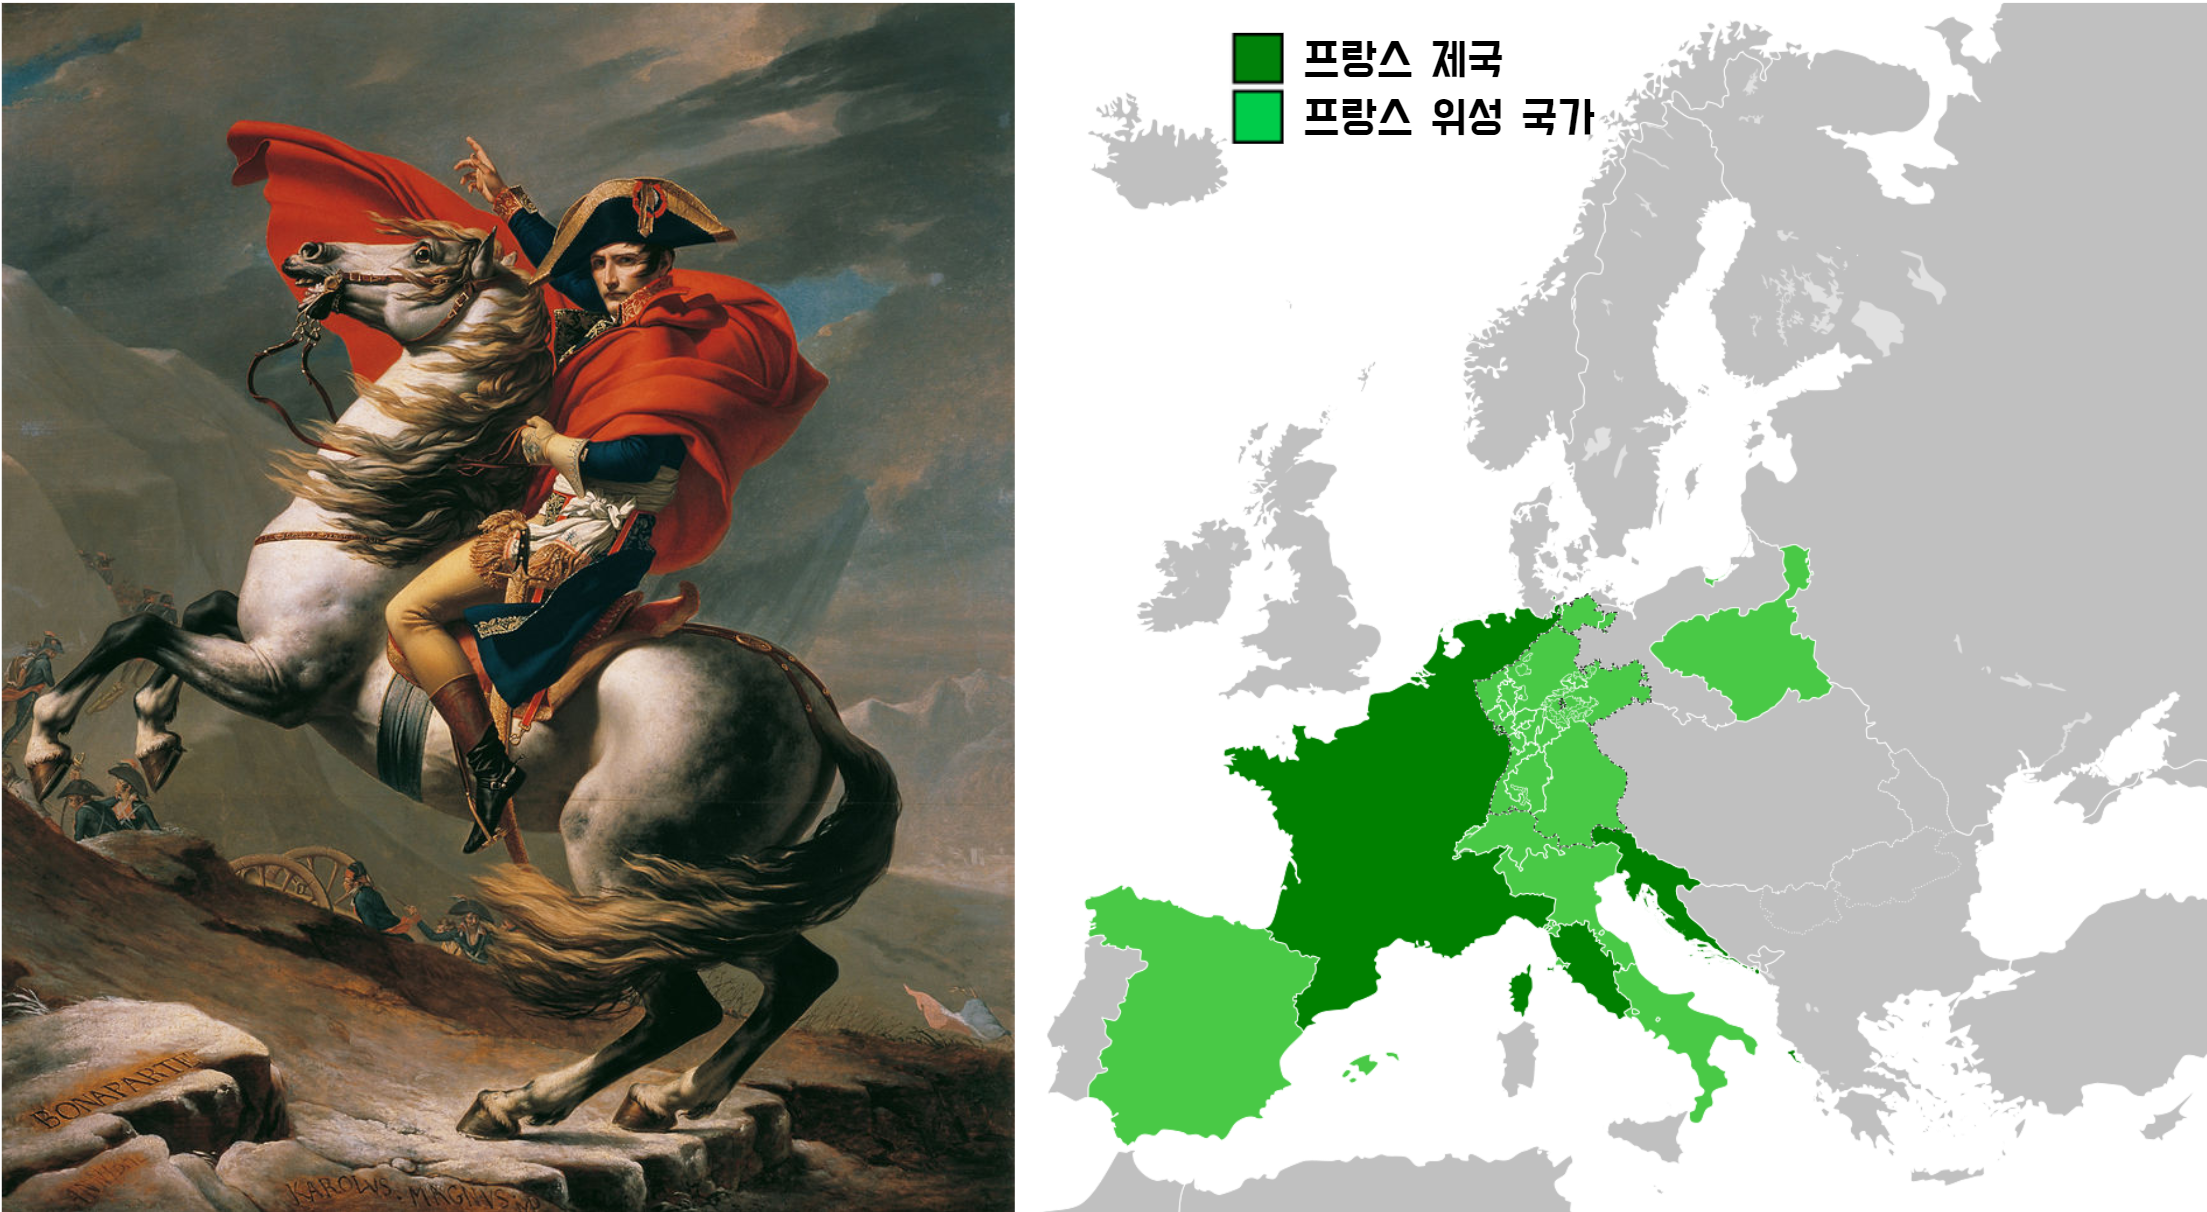
\includegraphics[width=1\textwidth,height=\textheight]{assets/images/about_napoleon.png}

최대 전성기를 구가하던 1812년 나폴레옹은 러시아 침공을 감행했다. 나폴레옹의
러시아침공은 데이터 시각화의 역작을 남기는 계기가 되기도 했다.
미나르는 프랑스의 러시아 침공을 군더더기 없이 시작부터 폐퇴하여 돌아온 과정까지 간략하게 표현했다.

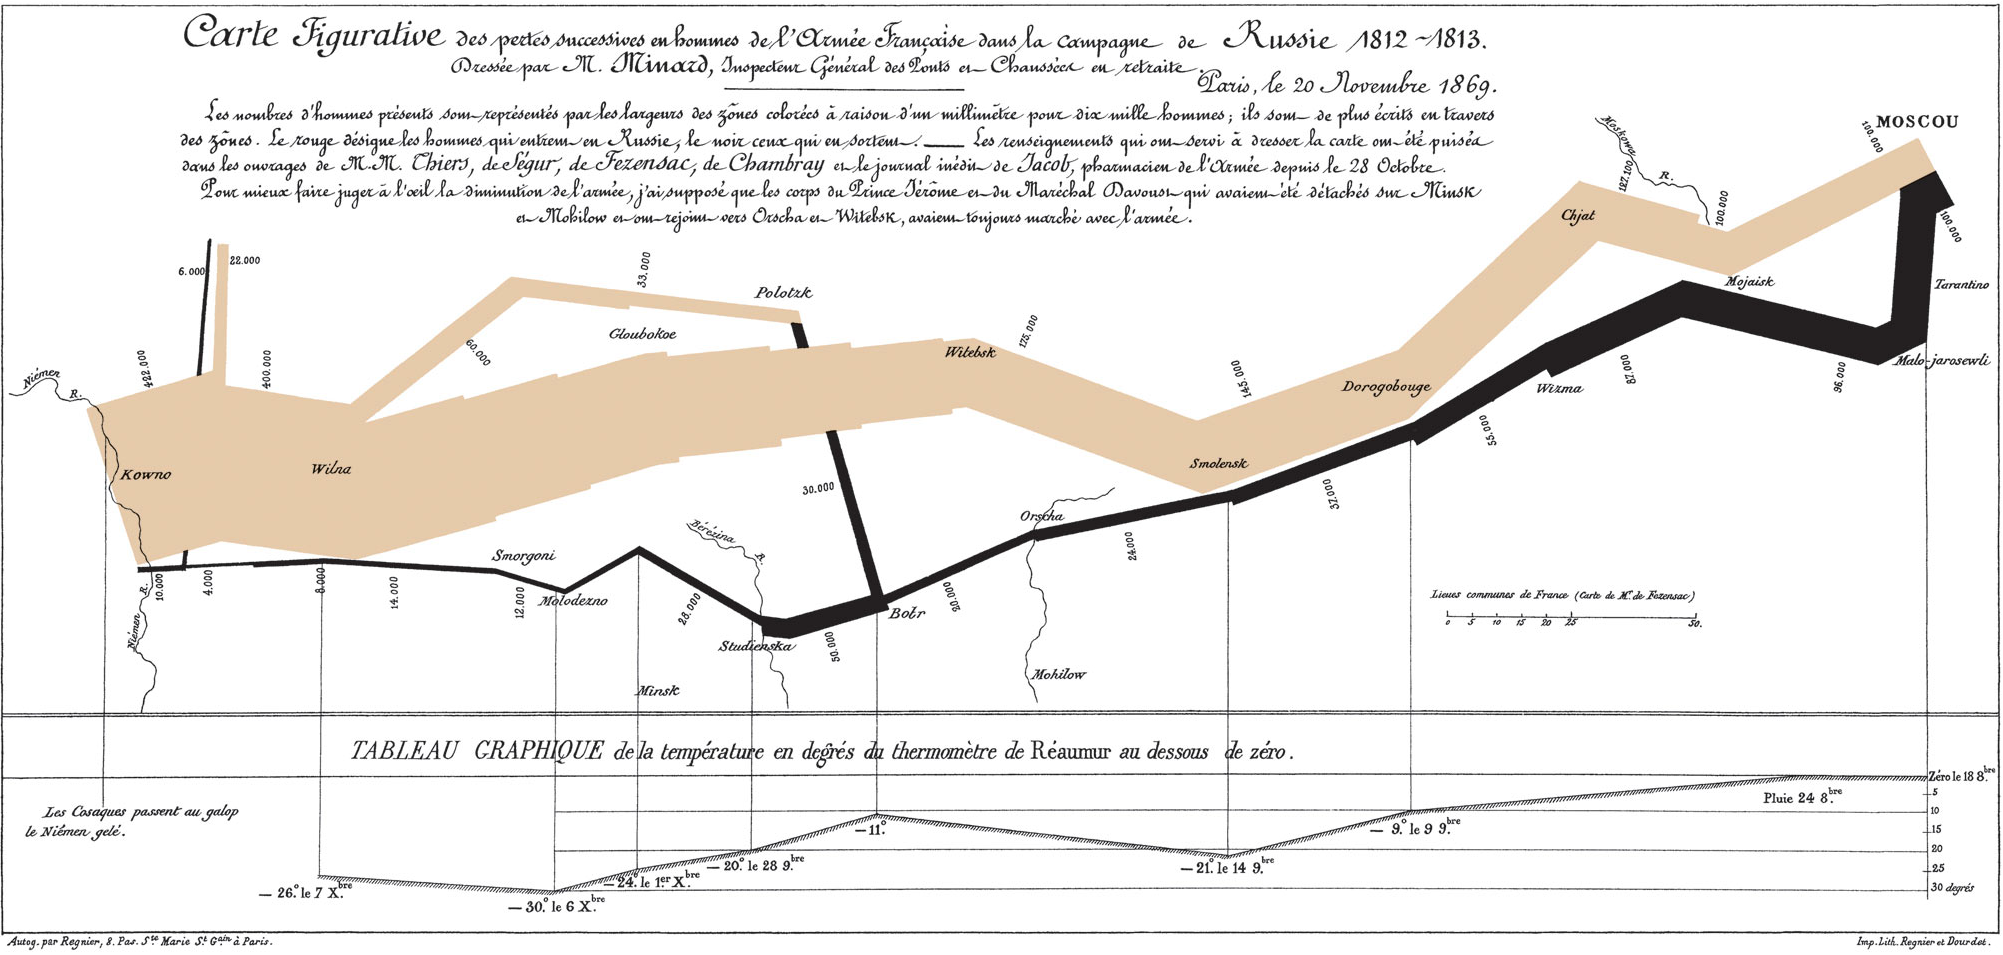
\includegraphics[width=1\textwidth,height=\textheight]{assets/images/Minard.png}

미나르 데이터 시각화의 지명을 자세히 보면 프랑스의 러시아 침공에 대해 대략적으로
인식하고 있는 것과 다소 차이가 난다. 통상 프랑스 수도 파리에서 나폴레옹 대군이
출발하여 러시아 모스코바에서 한동안 머물다가 다시 수도 파리로 돌아와서 황제에서
끌어내려져 엘바섬으로 위배를 떠난 것으로 알려져 있지만 실제 미나르가 데이터에
기반하여 제작한 시각화 그래프에는 진실이 담겨있다. \footnote{\href{https://theeducationalblog.quora.com/Why-did-Napoleon-s-Russian-campaign-end-in-failure-http-www-ryin-main-quora-com-Why-did-Napoleon-s-Russian-campaign}{Alexey Tereshchenko, ``Why did Napoleon's Russian campaign end in failure?'', Quora}}

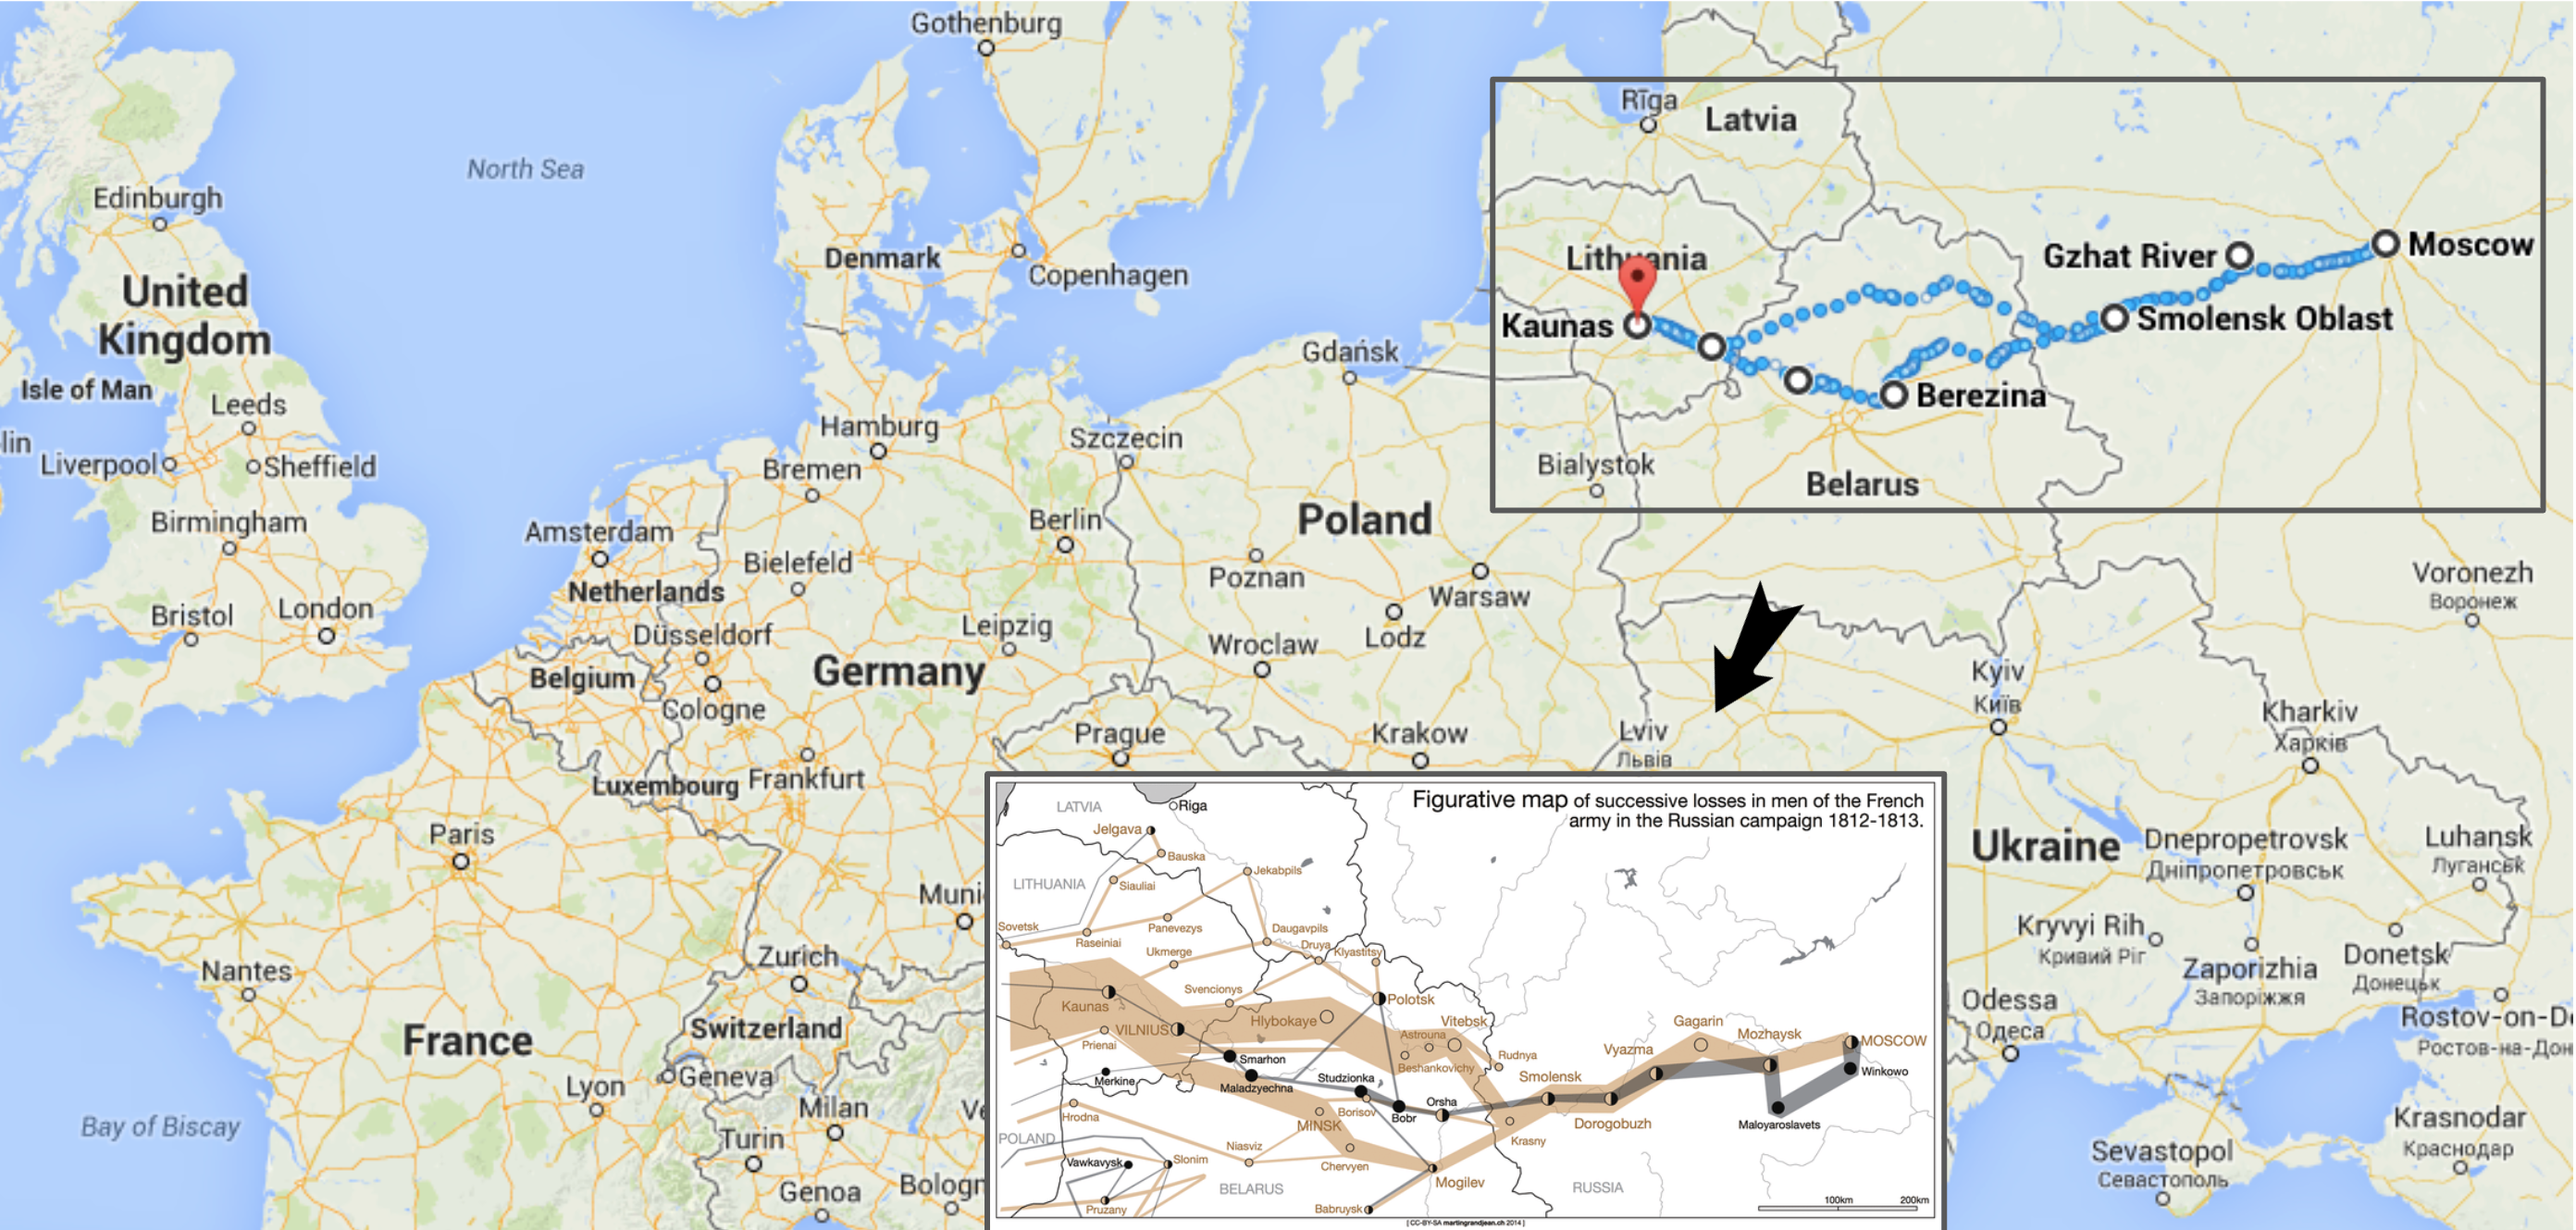
\includegraphics[width=1\textwidth,height=\textheight]{assets/images/minard-actual-map.png}

\hypertarget{napoleon-viz}{%
\section{시각화}\label{napoleon-viz}}

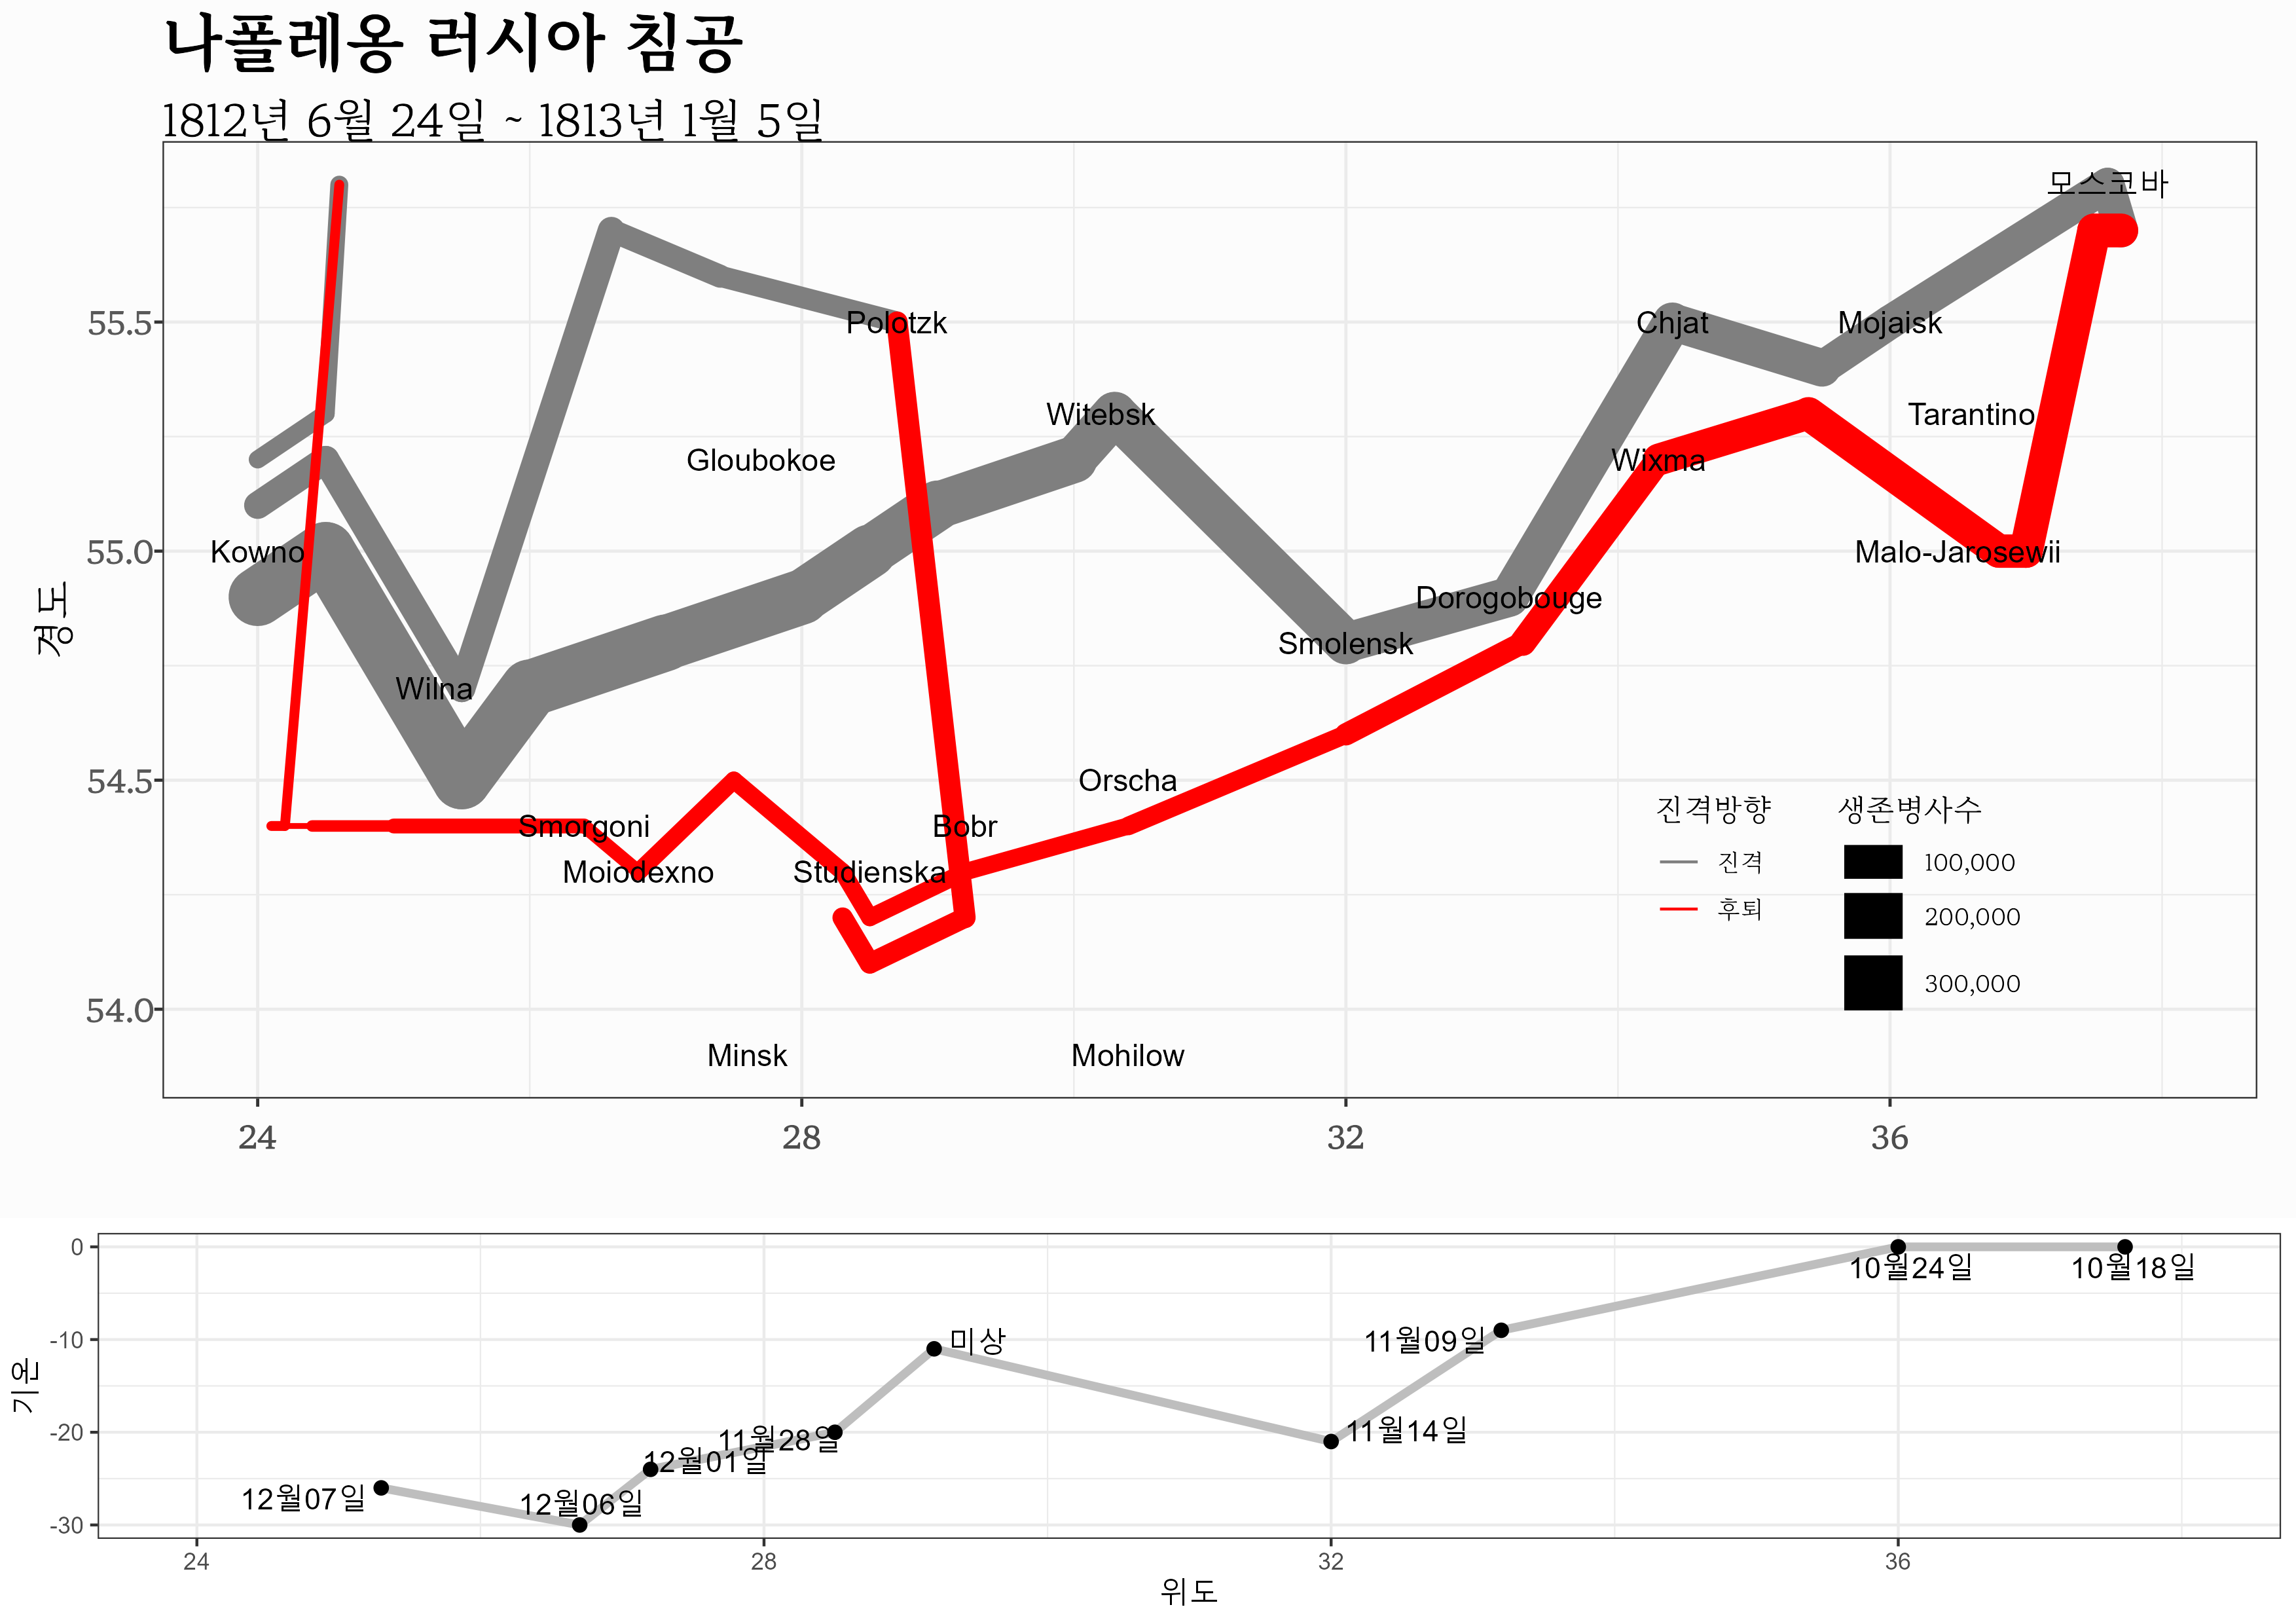
\includegraphics[width=1\textwidth,height=\textheight]{assets/images/나폴레옹_러시아.png}

\hypertarget{references}{%
\section{참고서적}\label{references}}

영어로 참고할 오픈 데이터 시각화 교재

\begin{itemize}
\tightlist
\item
  \citep{healy2018data}
\item
  \citep{dougherty2021hands}
\item
  \citep{wilke2019fundamentals}
\end{itemize}

\hypertarget{uxc2dcuxac01uxd654-uxad6cuxc131uxc694uxc18c}{%
\chapter*{시각화 구성요소}\label{uxc2dcuxac01uxd654-uxad6cuxc131uxc694uxc18c}}
\addcontentsline{toc}{chapter}{시각화 구성요소}

데이터 시각화를 할 때 다양한 구성요소를 이해하고 이를 체계적으로 조합하여
시각화 객체를 제작해야만 이후 재사용가능한 시각화 산출물을 제작하여 지속적인
발전을 이뤄낼 수 있다.

\hypertarget{viz-font}{%
\chapter{글꼴}\label{viz-font}}

R을 단순히 통계 언어로 생각하지 말고 적용범위를 확대해서 활용하면
데이터 과학 산출물을 다양한 전자문서로 제작하여 커뮤니케이션 할 수 있다.
PDF, HTML, 워드 등 문서 뿐만 아니라, 파워포인트 같은 발표자료를
슬라이드로 제작하여 배포할 수 있다. 그래프 문법(Grammar of Graphics)에 따라
\texttt{ggplot} 시각화를 산출물에도 다양한 글꼴(font)을 반영하여 좀더 관심을 끌 수 있는
그래프 제작도 가능하다. 데이터 과학자나 개발자 관점에서도 통합개발환경(IDE)이
필요한데 개발과 저작에 집중할 수 있는 글꼴을 지정하여 활용할 경우
생산성도 높일 수 있고 좀더 쾌적한 환경에서 개발을 진행할 수 있다.

R 스크립트 작성을 위한 글꼴과 그래프에 한글 글꼴(font)을 적용한다.
\texttt{ggplot}을 비롯한 시각화를 위해 \texttt{extrafont}와 \texttt{showtext} 패키지를
활용하여 적절한 한글 글꼴을 사용할 뿐만 아니라 코딩 개발할 때
R 스크립트(\texttt{.R}) 및 R마크다운(\texttt{.Rmd})에서도 적절한 한글글꼴 사용을 위해서
코딩관련 글꼴도 설치한다.

기본적인 작업흐름은 운영체제에 먼저 외부에서 가져온 폰트를 설치한다.
그리고 나서 \texttt{extrafont} 팩키지 \texttt{font\_import()} 함수를 사용해서 폰트를
R에서 불러 사용할 수 있도록 설치한다. 그리고 나서 \texttt{loadfonts()} 함수를
사용해서 글꼴을 \texttt{ggplot}등에서 불러 사용한다.
\href{https://fonts.google.com/}{구글 글꼴}을 사용하고자 할 경우 \texttt{showtext} 패키지를
사용해서 로컬 컴퓨터에 설치하여 적용한다.

\begin{figure}
\centering
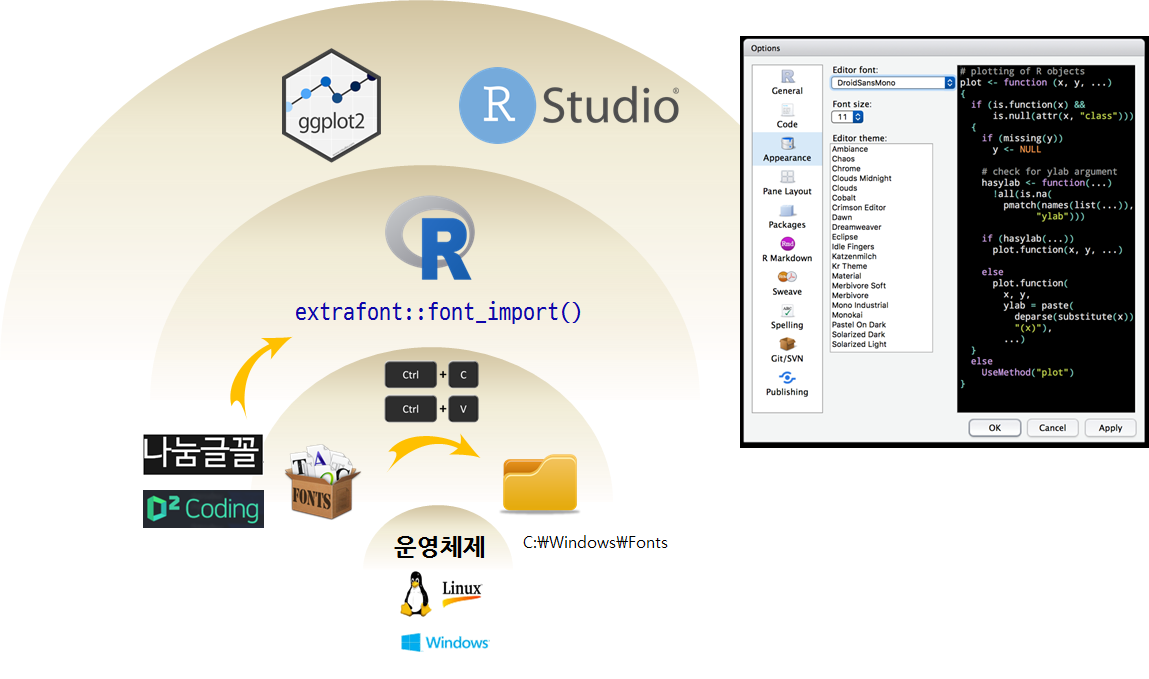
\includegraphics[width=1\textwidth,height=\textheight]{assets/images/font_overview.png}
\caption{R 폰트/글꼴 설치}
\end{figure}

\hypertarget{font-coding}{%
\section{R 코딩 글꼴}\label{font-coding}}

문서를 위해 작성하는데 사용되는 글꼴과 R 코딩을 위해 사용되는 글꼴은
차이가 난다. 왜냐하면 R 코딩에 사용되는 글꼴은 가독성이 좋아야하고
디버깅에 용이해야 된다. 영어는 \texttt{consolas} 글꼴을 많이 사용하는데 무료가
아니다. 그래서 \texttt{consolas}에서 영감을 받은 SIL 오픈 폰트 라이선스를
따르는 \href{https://en.wikipedia.org/wiki/Inconsolata}{Inconsolata}가 R
코딩에 많이 사용되고 있다. 하지만, R코드를 작성할 때 주석을 한글로
달거나 R마크다운 작업을 할 경우 유사한 기능을 하는 한글 글꼴이 필요하다.

\begin{itemize}
\tightlist
\item
  \href{https://github.com/naver/nanumfont/blob/master/README.md}{네이버 나눔고딕 코딩글꼴}
\item
  \href{https://github.com/naver/d2codingfont}{D2 Coding 글꼴}
\end{itemize}

``네이버 나눔고딕 코딩글꼴''과 ``D2 Coding 글꼴''을 설치하고 나서 RStudio
IDE에서 ``Tools'' → ``Global Options\ldots{}''를 클릭하면 ``Options''창에서
\texttt{Appearance}에서 \textbf{Editor font:}에서 설치한 코딩전용 글꼴을 선택하고
\textbf{Editor theme:}도 지정한다.

\begin{figure}
\centering
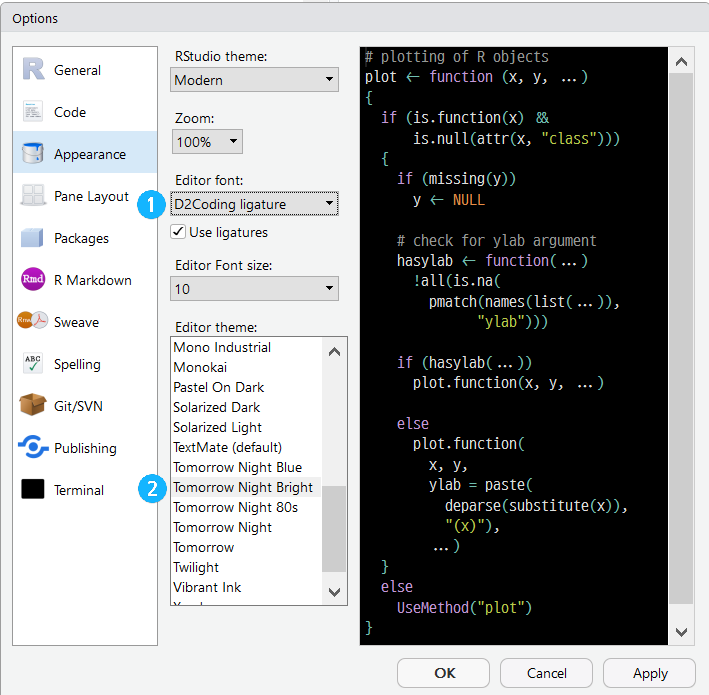
\includegraphics[width=1\textwidth,height=\textheight]{assets/images/font_d2coding.png}
\caption{D2 코딩폰트 설치}
\end{figure}

\hypertarget{r-viz-font}{%
\section{\texorpdfstring{\texttt{ggplot} 시각화 글꼴}{ggplot 시각화 글꼴}}\label{r-viz-font}}

\texttt{extrafont} 팩키지에서 \texttt{font\_import()} 함수로 운영체제(윈도우/리눅스)에
설치된 글꼴을 R로 가져온다. 그리고 나서 \texttt{loadfonts()} 함수를 사용해서
설치된 글꼴을 사용하는 작업흐름을 따르게 된다.

\hypertarget{font-viz-font-example}{%
\subsection{\texorpdfstring{\texttt{ggplot} 한글 글꼴 사례}{ggplot 한글 글꼴 사례}}\label{font-viz-font-example}}

\texttt{extrafont} 패키지 \texttt{loadfonts()} 함수를 사용해서 \texttt{ggplot}에서 적용시킬 수 있는
글꼴을 불러냈다. R 내장 데이터셋 \texttt{iris}를 사용하여 나눔글꼴 ``Nanum Pen Script''을 기본 글꼴로 적용시켰다.

\begin{center}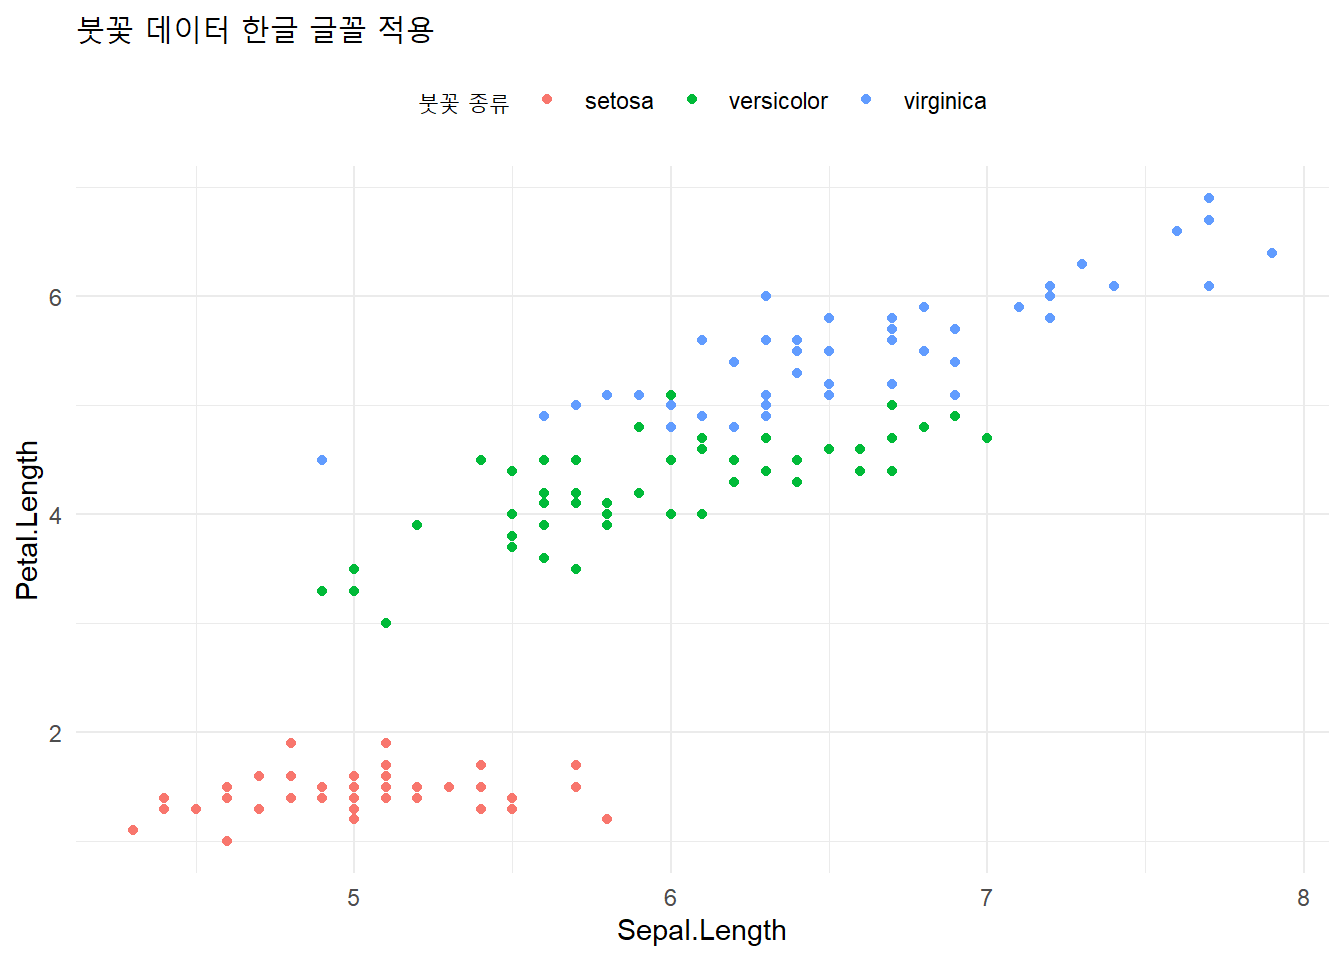
\includegraphics{basics-font_files/figure-latex/ggplot-extrafont-in-r-1} \end{center}

\hypertarget{font-showtext}{%
\section[\texttt{showtext} 패키지 ]{\texorpdfstring{\texttt{showtext} 패키지 \footnote{\href{https://cran.rstudio.com/web/packages/showtext/index.html}{showtext: Using Fonts More Easily in R
  Graphs}}}{showtext 패키지 }}\label{font-showtext}}

\href{https://github.com/wch/extrafont}{extrafont} 패키지를 통해 한자를
포함한 한글을 처리할 수 있었으나, \href{https://github.com/wch/extrafont}{extrafont}는 트루타입폰트(\texttt{.ttf})를
PDF 그래픽 장치에 초점을 맞춰 개발이 되었다. 따라서, 데이터과학
최종산출물이 PDF 형태 책이 아닌 경우 여러가지 면에서 다양한 한글 글꼴을
표현하는데 있어 한계가 있다.

새로 개발된 \href{https://cran.rstudio.com/web/packages/showtext/index.html}{showtext}
팩키지는 \texttt{Ghostscript}같은 외부 소프트웨어를 활용하지 않고도 다양한
(그래픽) 글꼴을 지원한다. \href{https://cran.rstudio.com/web/packages/showtext/index.html}{showtext}로
R 그래프를 생성할 때, 다양한 글꼴(TrueType, OpenType, Type 1, web fonts
등)을 지원한다.

과거 PDF와 같은 책형태로 정보를 공유하고 전달하는 방식이 주류를 이뤘다면
인터넷 등장 이후 웹으로 정보 생성과 소비가 주류로 떠오르게 되면서 글꼴에도
변화가 생겼다. 가까운 미래에는 웹을 우선시하는 글꼴이 대세를 이룰 것으로 보인다.

\begin{figure}
\centering
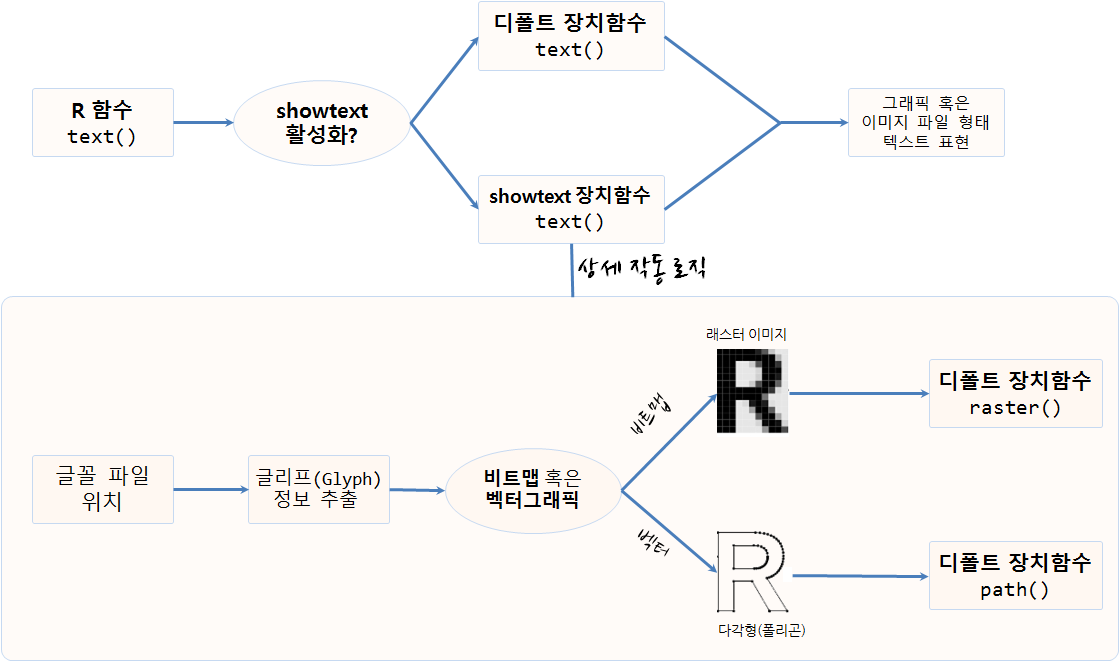
\includegraphics[width=1\textwidth,height=\textheight]{assets/images/font-showtext.png}
\caption{\texttt{showtext} 글꼴}
\end{figure}

사용자가 그래프에 텍스트를 넣기 위해 R 함수에서 \texttt{text()}를 호출할 때
\texttt{showtext}가 활성화 되어 있으면 \texttt{showtext} 팩키지 \texttt{text()} 함수를
호출해서 그래픽 혹은 이미지 파일에 텍스트를 표현하고 그렇지 않는 경우는
디폴트 장치함수 \texttt{text()} 함수를 호출하게 되어 있다.

내부적으로 상세 작동 로직은 글꼴 위치를 파악해서 글리프(glyph) 정보를
추출하고 비트맵 형식, 벡터그래픽 형식에 따라서 비트맵일 경우 \texttt{raster()}
장치함수를 호출하고, 벡터그래픽인 경우 \texttt{path()} 장치함수를 호출해서
기능을 수행한다.

\hypertarget{showtext-korean-example}{%
\subsection{R 설치 글꼴 확인}\label{showtext-korean-example}}

\texttt{extrafont} 팩키지 \texttt{loadfonts()} 함수를 통해 \texttt{.ttf} 파일 정보를
확인한다. 현재 \href{http://www.google.com/fonts}{구글 글끌} 페이지에서 많은 한글
글꼴을 지원하지 않고 있다. 구글에서 전세계 글꼴을 지원하다보 동아시아 3국 대상으로
지원되는 글꼴은 적은 것으로 보인다.

\hypertarget{font-showtext-korean-example-ggplot}{%
\subsection{\texorpdfstring{\texttt{ggplot} 글꼴 적용}{ggplot 글꼴 적용}}\label{font-showtext-korean-example-ggplot}}

한글 글꼴을 바로 적용하기에 앞서 \texttt{showtext} 패키지 포함된 영문글꼴 적용 사례를 먼저 돌려보자.
\texttt{ggplot} 그래픽에 적용되는 \texttt{showtext} 활용 기본 작업흐름은 다음과 같다.

\begin{enumerate}
\def\labelenumi{\arabic{enumi}.}
\tightlist
\item
  글꼴을 적재한다.
\item
  그래픽 장치를 연다
\item
  \texttt{showtext}를 통해 텍스트를 표시한다고 지정한다.
\item
  그래프를 그린다.
\item
  장치를 닫는다.
\end{enumerate}

\hypertarget{font-showtext-korean-example-ttf}{%
\section{로컬 글꼴 적용}\label{font-showtext-korean-example-ttf}}

로컬 컴퓨터에 저장된 \texttt{.ttf} 파일을 사용자 지정해서 가져온 후 이를
\texttt{ggplot}에 반영하여 한글을 R 그래프에 적용하는 것도 가능하다.
\texttt{showtext}는 \texttt{extrafont} 보다 나중에 개발되어 \texttt{extrafont}가
로컬 컴퓨터에 설치된 글꼴을 \texttt{ggplot}에 구현되는데 전력을 다했다면
\texttt{showtext}는 이를 발판으로 나중에 개발되어 구글 폰트와 같은
인터넷 글꼴과 최근 웹출판에 대한 개념도 넣어 개발된 것이 차이점이다.

\hypertarget{ggplot-component}{%
\chapter{구성요소}\label{ggplot-component}}

깔끔한 데이터(tidy data)가 준비되면 이를 시각화하기 위해서는 데이터를 시각화 객체에 매핑하게 되는 메커니즘이 필요하다.
주요 구성요소로 시각적 매핑(Aesthetics), 척도(Scale), 좌표계(Coordiate System), 축(Axis) 등이 필요하다.

\hypertarget{ggplot-aesthetics}{%
\section{시각적 매핑(Aesthetics)}\label{ggplot-aesthetics}}

\texttt{ggplot}에서 시각적 매핑(Aesthetics)는 \texttt{aes()} 내에 시각적으로 표현되는 모든 것을 담고 있다.
시각화 대상은 크게 두가지로 나눠지는데 연속형과 범주형이다. 온도나 몸무게 같은 경우는 특정 두 데이터 값 사이 연속된 값이 있지만,
수학에서 정수와 같이 표현되는 쪼갤 수 없는 경우는 국가를 생각하면 한국과 미국 사이 존재하는 값이 없다.
시각화를 할 경우 위치(position), 모양(shape), 크기(size), 색상(color), 선굵기(line width), 선유형(line type)을 사용하여 좌표계(coordinate system), 척도(scale)와 결합하여 최종 시각화 결과물을 제작된다. Claus Wilke 시각화 책에 언급된 다양한 시각적 매핑을 통해 효과적으로 데이터의 정보를 표현할 수 있다.\citep{wilke2019fundamentals} 당연히 위치, 모양, 크기, 색상, 선굵기, 선유형 중 어떤 것을 사용하느냐에 따라 시각화로 전달되는 정보의 양은 달라진다. 예를 들어, 위치는 시각적 변별력이 선 유형보다 크다.

\begin{figure}

{\centering 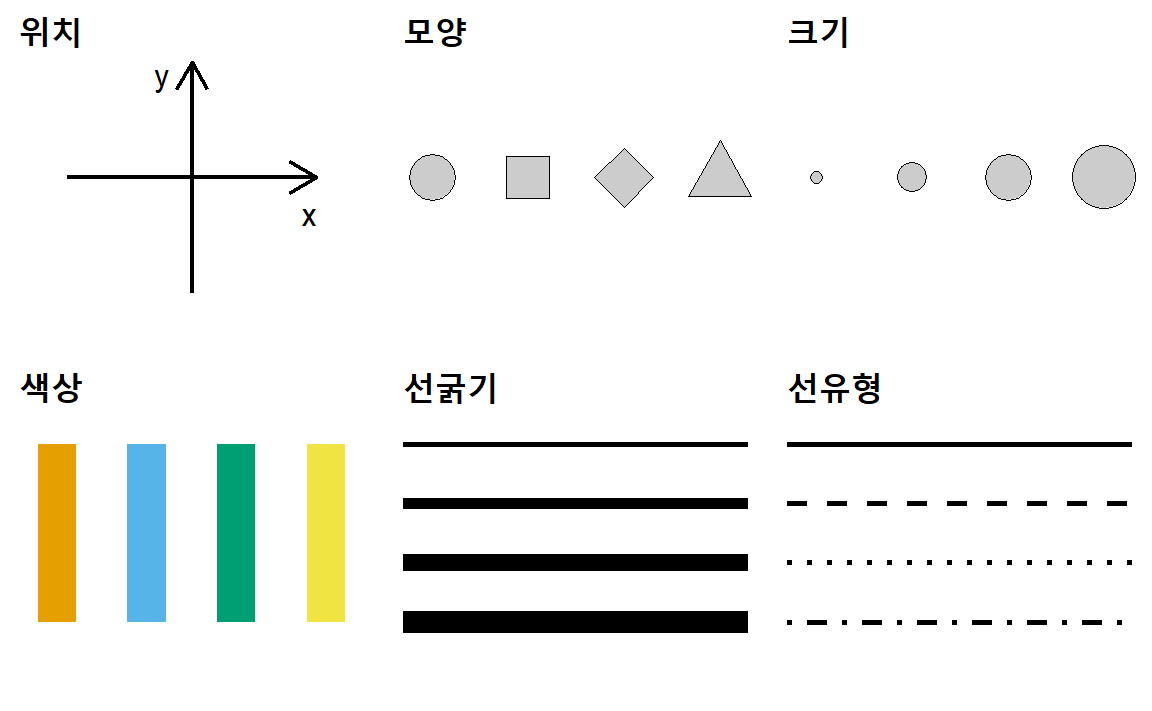
\includegraphics{basics-component_files/figure-latex/ggplot-six-aesthetics-1} 

}

\caption{위치, 모양, 크기, 색상, 선굵기, 선유형 등 시각적 매핑}\label{fig:ggplot-six-aesthetics}
\end{figure}

\hypertarget{scale-mapping}{%
\section{척도 매핑}\label{scale-mapping}}

데이터가 주어지면 시각적 객체(모양, 색상, 크기 등)와 매핑을 해야 되는데 그 둘 사이를 연결하는 것이 척도(Scale)이다.
\texttt{x}축과, \texttt{y}축 척도에 시각적 객체를 매핑해야 비로서 데이터 값을 그래프로 표현된다.
척도에 위치가 지정되면 시각적 매핑 객체를 다양하게 표현할 수 있다. 만약 위치가 척도에 모호하게 표현되게 되면
시각적 객체가 제대로 그래프에 표현되는데 문제가 된다.

\begin{figure}

{\centering 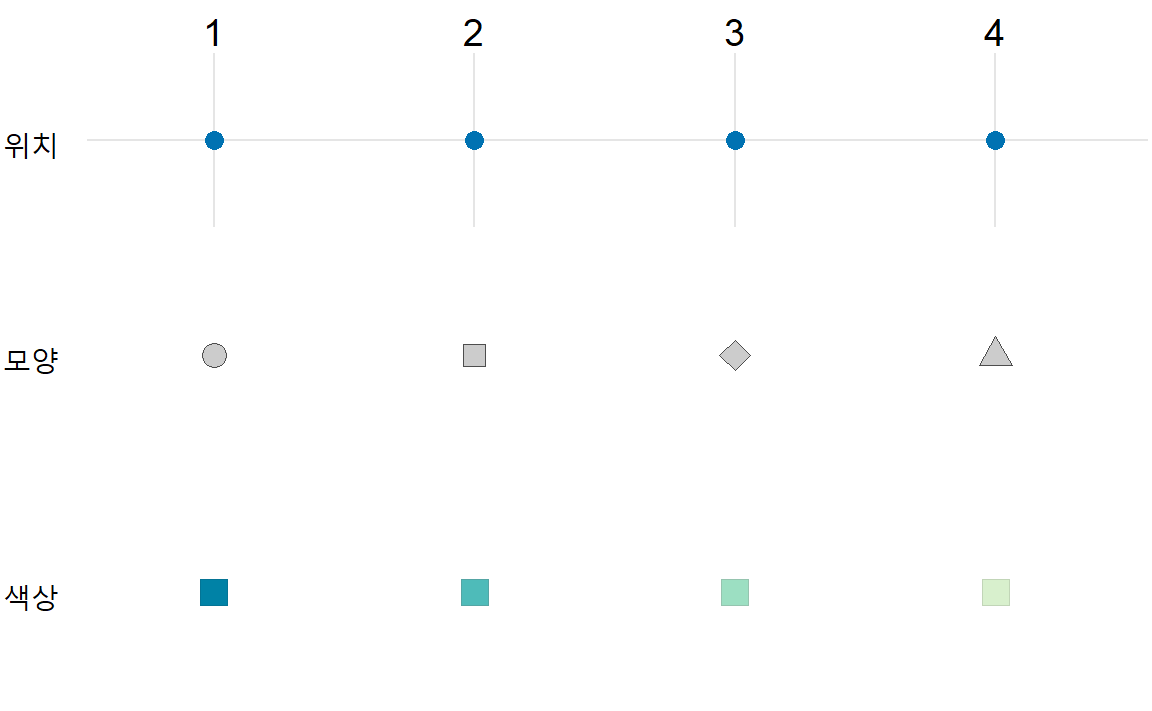
\includegraphics{basics-component_files/figure-latex/ggplot-scale-1} 

}

\caption{시각적 객체 척도 매핑}\label{fig:ggplot-scale}
\end{figure}

\hypertarget{coordinate}{%
\section{좌표계}\label{coordinate}}

데이터 시각화에서 앞서 데이터를 척도와 시각적 객체로 준비를 했다면 이를 최종 그래프로 제작하기 위해서는 좌표계가 필요하다.
네이버 사전에서 좌표계는 공간상의 한 점의 위치를 표시하는 숫자들의 순서쌍인 좌표를 정하기 위한 체계로서, 원점과 기준 길이, 기준 축이나 기준선들의 집합을 통틀어 이르는 말이다. 가장 널리 사용되는 좌표계는 데카르트 직각좌표계와 극좌표계가 널리 사용된다.
다음은 \texttt{mtcars} 데이터 차량 기통수를 막대그래프와 원그래프를 사용하여 동일한 내용을 좌표계만 달리하여 시각적으로 표현해따.

\begin{figure}

{\centering 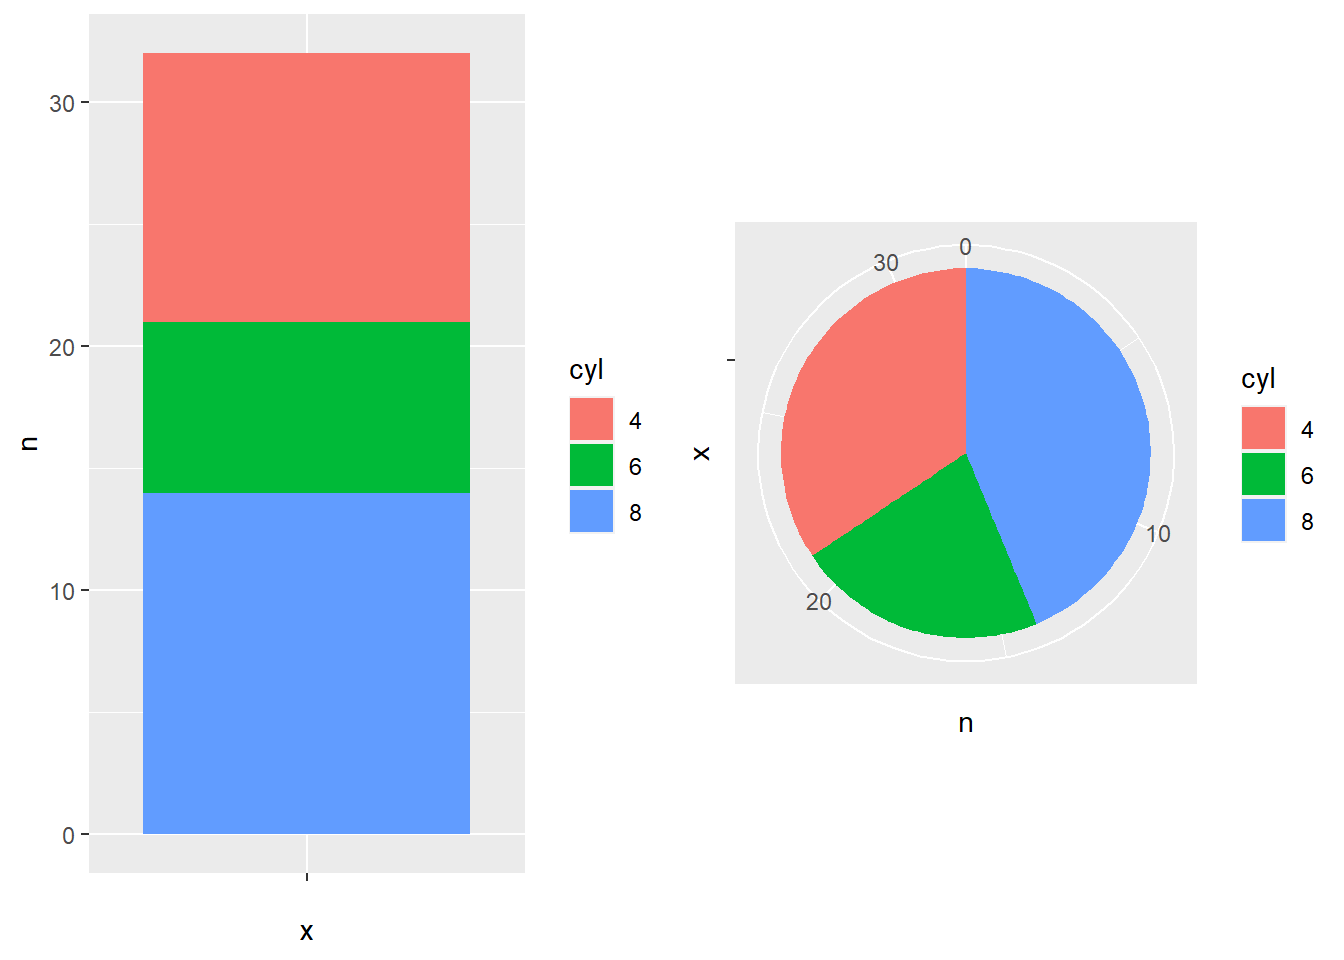
\includegraphics{basics-component_files/figure-latex/ggplot-coordinate-1} 

}

\caption{직교좌표계와 극좌표계}\label{fig:ggplot-coordinate}
\end{figure}

\hypertarget{coordinate}{%
\section{축(axis)}\label{coordinate}}

데이터 값을 선형 척도에 매핑하여 시각화하는 것이 일반적이지만 \texttt{x,\ y} 축이
대표적으로 날짜와 같은 시계열 데이터인 경우 혹은 시분초를 나타내는 경우도 있어 이에 맞춰
적절히 축을 맞춰야 한다. 덧셈이 아니라 곱셈에 대해 선형인 경우 로그변환을 취하여
데이터 본연의 척도를 반영하도록 축을 조정한다. 많이 사용되는 로그 변환의 경우
밑을 10으로 하는 상용로그와 자연로그가 있어 명확히 축라벨에 적시하여 혼동을 피하는 것이 좋다.
로그 변환시 \textbf{0}이 있는 경우 문제가 되기 때문에 \texttt{sqrt()} 변환도 로그변환이 갖는 표현법의 장점을
갖추면서도 로그변환 시 생기는 번거러움을 해소하기 자주 사용된다.

\begin{figure}

{\centering 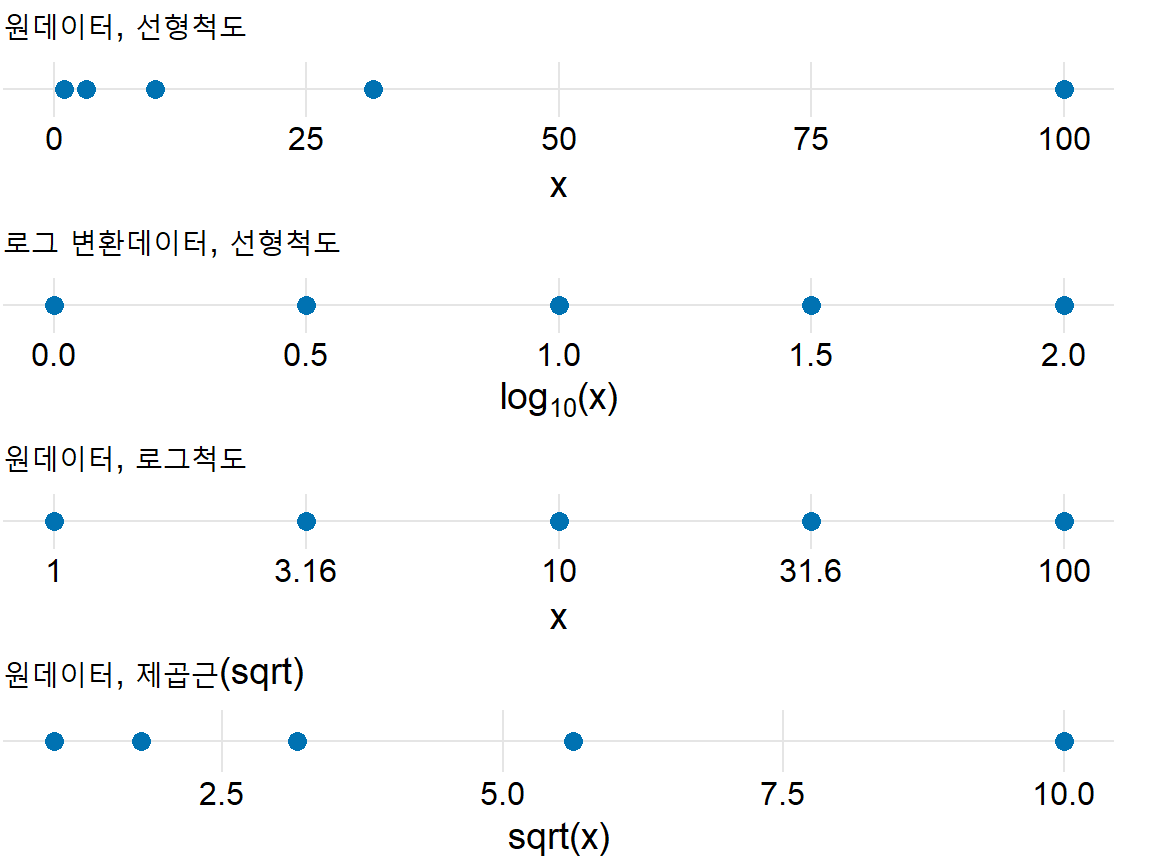
\includegraphics{basics-component_files/figure-latex/linear-log-scales-1} 

}

\caption{선형, 로그, 제곱근 축}\label{fig:linear-log-scales}
\end{figure}

\hypertarget{uxc2dcuxac01uxd654}{%
\chapter*{시각화}\label{uxc2dcuxac01uxd654}}
\addcontentsline{toc}{chapter}{시각화}

\hypertarget{ggplot}{%
\chapter{그래프 문법}\label{ggplot}}

\hypertarget{why-ggplot2}{%
\section{그래프 문법의 존재이유}\label{why-ggplot2}}

Leland Wilkinson의 ``The Grammar of Graphics''는 1999년 첫 출간된 이후 \textbf{데이터 그래픽(data graphics)}에 많은 영향을 주어 \texttt{ggplot2}, Polaris → Tableau, Vega-Lite 등의 형태로 우리곁에 다가섰다.
기존 데이터를 시각화한 다양한 그래픽 객체를 만드려면 각 그래픽 객체별로 따로 사용법을 익혀야만 되었다.
이것이 갖는 한계는 그래프 종류가 적은 경우 유용하지만 그래프 종류가 많아지면 매번 따로 사용법을 배워야되서
확장가능성이 무척 떨어지게 된다.
그래서, 이를 일반화한 무언가 필요한데 데이터 그래픽 객체를 분해해서 8개 계층으로 분해하여 조립하여
그래프를 제작하게 되면 앞선 문제를 일거에 해소할 수 있다.
\textbf{그래프 문법(grammar of graphics)}을 통해 데이터를 가장 잘 표현할 수 있는 그래프를 생성할 수 있게 되었다.

\begin{figure}
\centering
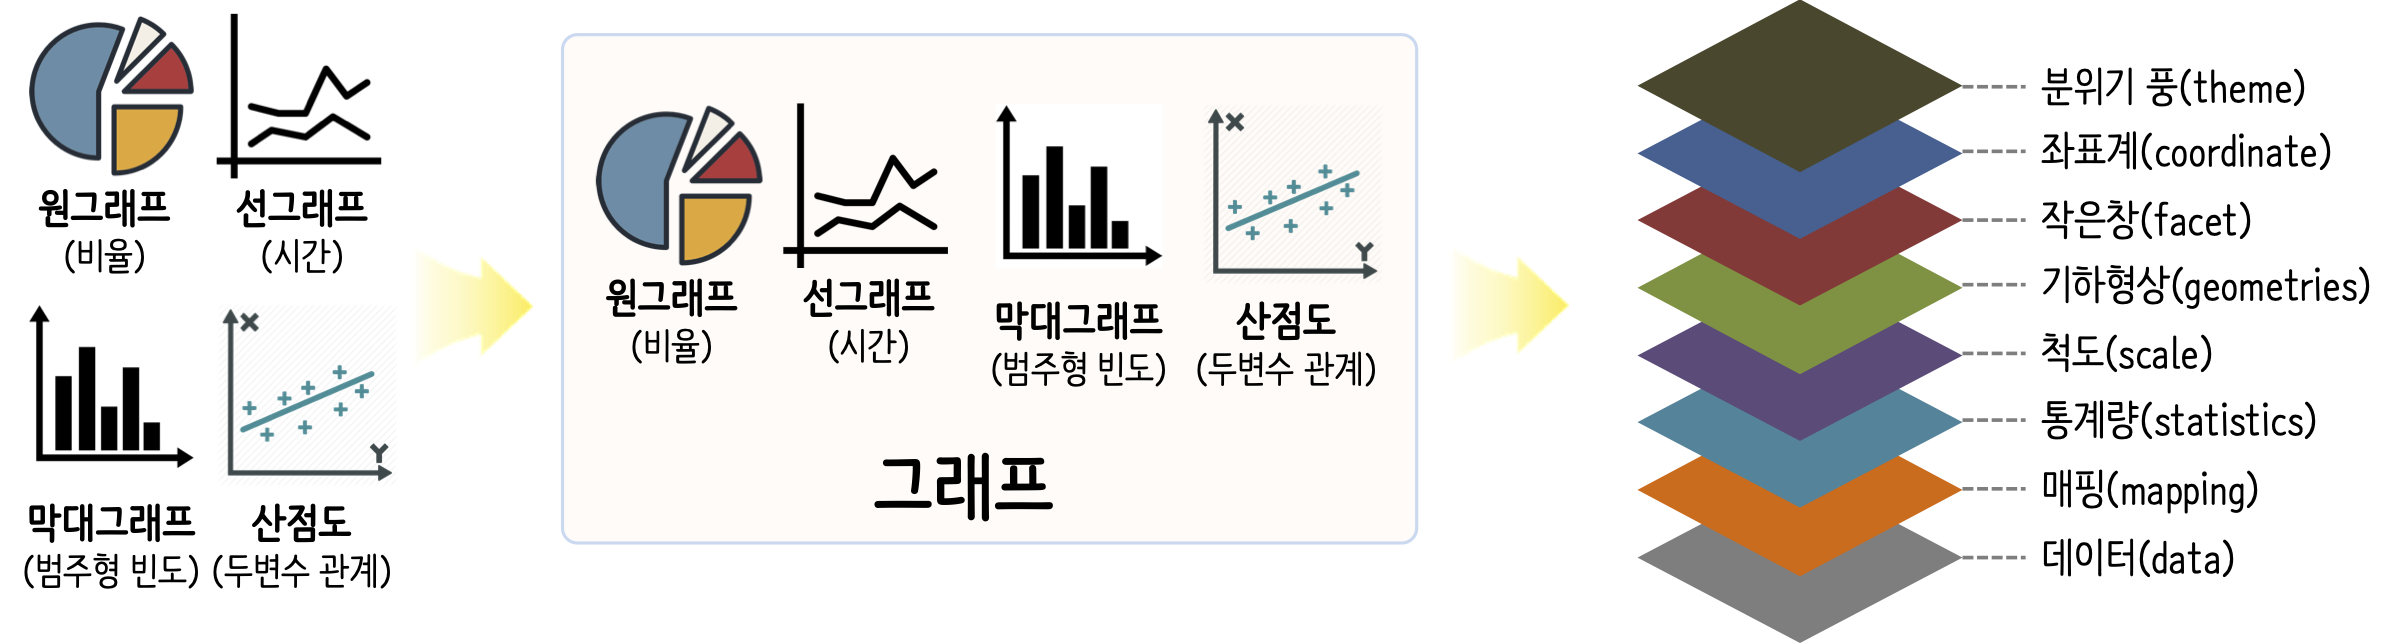
\includegraphics[width=1\textwidth,height=\textheight]{assets/images/ggplot_why.png}
\caption{\texttt{ggplot}이 필요한 이유}
\end{figure}

\hypertarget{ggplot2-steps}{%
\section{그래프 문법}\label{ggplot2-steps}}

그래프 문법은 총 8가지 층으로 구성되어 있는데 이를 각 층별로 나눠보면 다음과 같다.

\hypertarget{ggplot2-steps-data}{%
\subsection{데이터(Data)}\label{ggplot2-steps-data}}

그래프 문법 \texttt{ggplot}에 데이터는 깔끔한 데이터(tidy data)를 가정한다. 이를 위해서 기존 \texttt{wide}형태 데이터는 key-value \texttt{long} 형태로 바뀌어 준비한다.

\begin{figure}
\centering
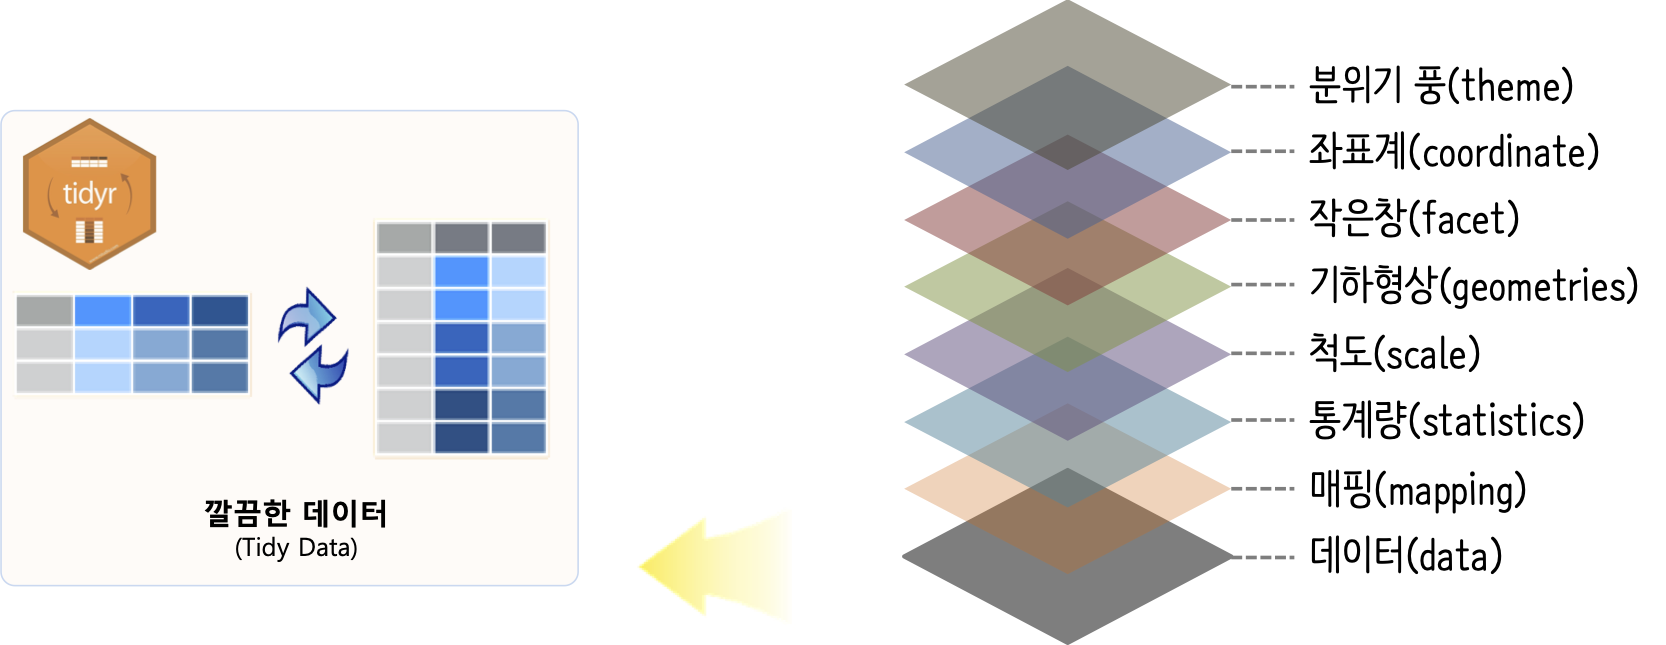
\includegraphics[width=1\textwidth,height=\textheight]{assets/images/ggplot-data.png}
\caption{깔끔한 데이터 \texttt{wide}, \texttt{long} 데이터}
\end{figure}

\hypertarget{ggplot2-steps-mapping}{%
\subsection{매핑(Mapping)}\label{ggplot2-steps-mapping}}

깔끔한 데이터가 준비되면 다음 단계로 칼럼에 해당되는 각 변수를 \texttt{aes()} 함수를 사용해서 \texttt{aes(x=x,\ y=y,\ color=z,\ ...)}와 같은 방식으로 데이터와 그래프를 매핑한다.

\begin{figure}
\centering
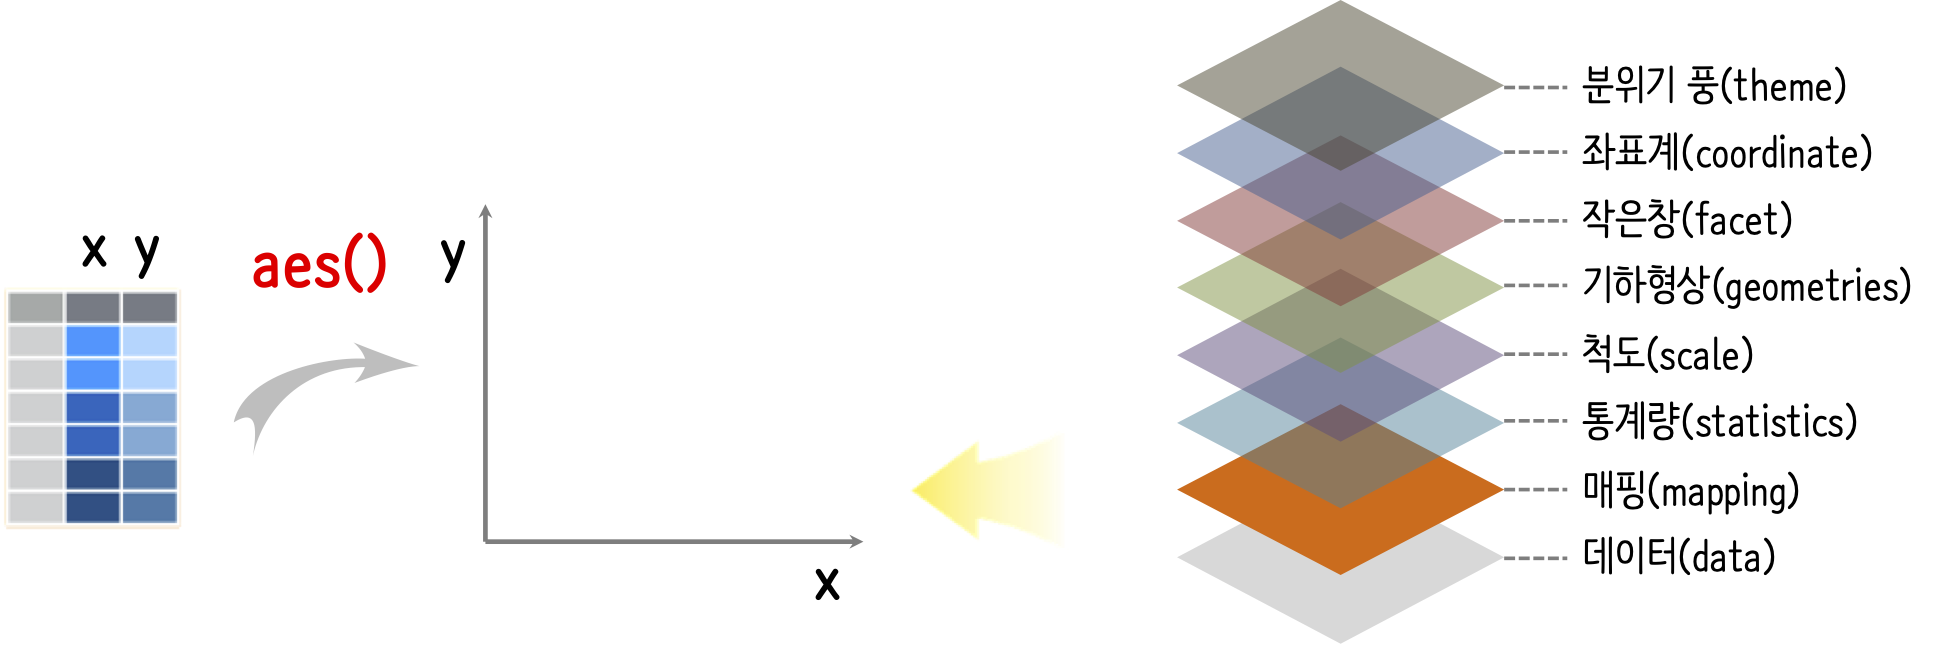
\includegraphics[width=1\textwidth,height=\textheight]{assets/images/ggplot-mapping.png}
\caption{데이터를 그래프에 매핑}
\end{figure}

\hypertarget{ggplot2-steps-statistics}{%
\subsection{통계량(statistics)}\label{ggplot2-steps-statistics}}

범주형 그래프를 시각화할 경우 빈도수를 통계량으로 계산해놔야 하고, 연속형 변수를 히스토그램으로 표현할 때도 마찬가지 방식으로 구간별 빈도수를 계산해놔야 하고, 특히 상자그림(boxplot)을 시각화할 경우 각 분위수는 물론이고 중위수도 및 interquantile도 계산해서 수염의 끝도 계산해놔야 제대로된 상자그림을 시각화할 수 있다.

\begin{figure}
\centering
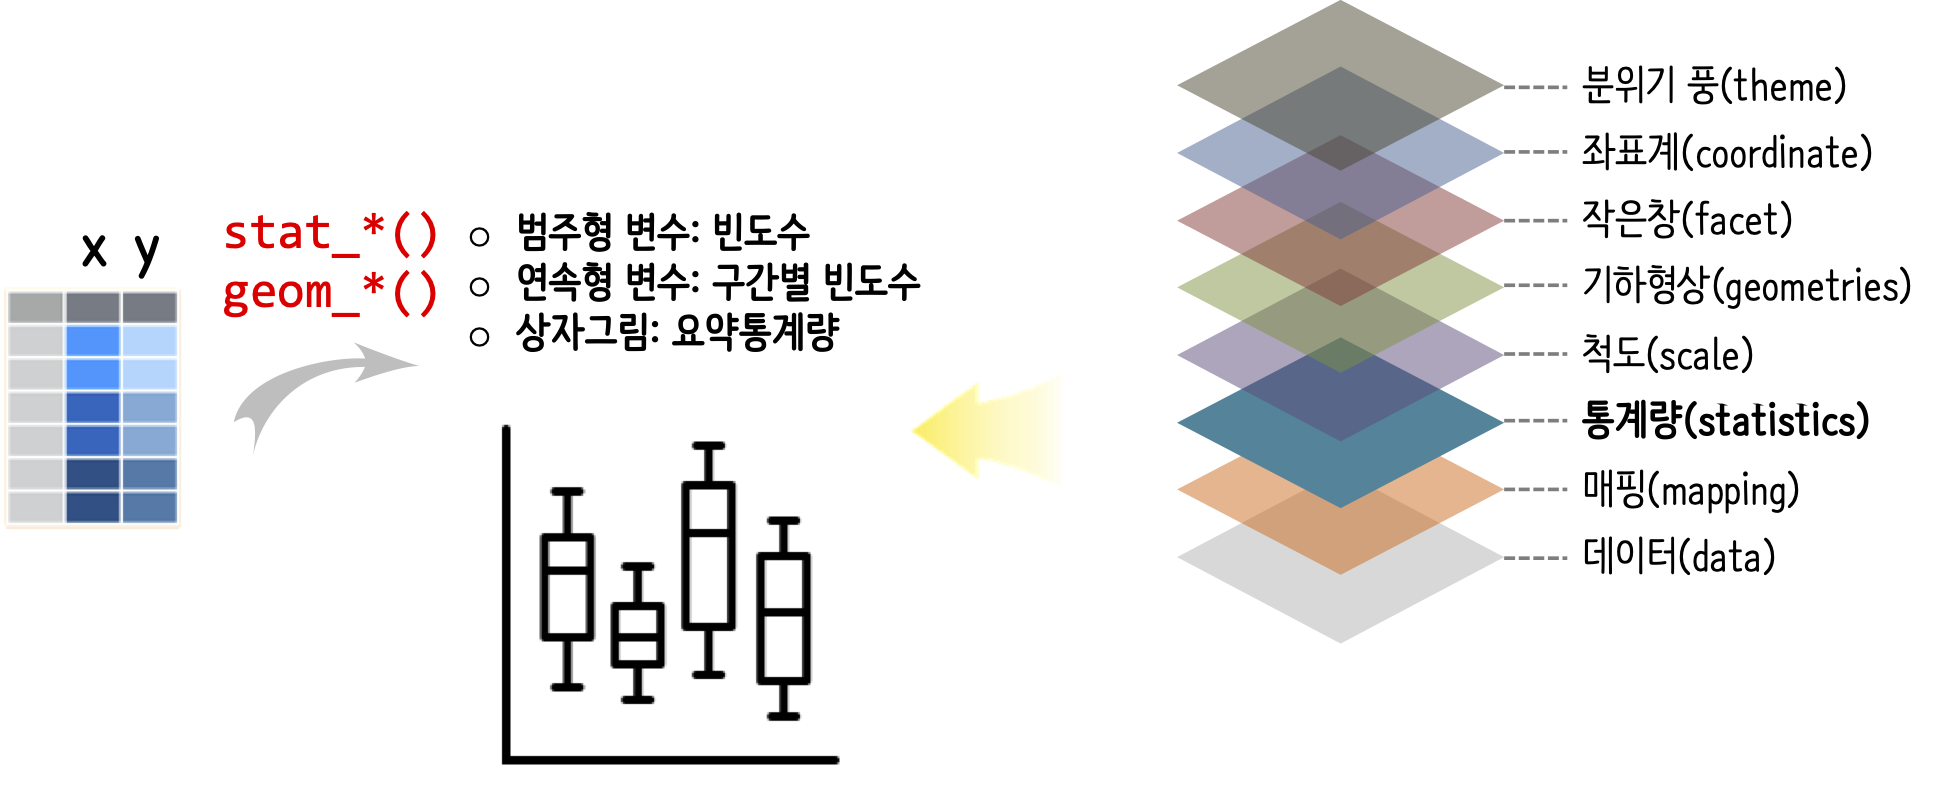
\includegraphics[width=1\textwidth,height=\textheight]{assets/images/ggplot-stat.png}
\caption{그래프별 기본설정 통계량}
\end{figure}

\hypertarget{ggplot2-steps-scales}{%
\subsection{척도(scales)}\label{ggplot2-steps-scales}}

X축, Y축의 척도를 그래프에서 자동으로 인식하는데는 한계가 있어 이를 필요한 경우 적절한 형태로 설정한다. \texttt{scale\_\textless{}x,\ y,\ color,\ fill,\ ...\textgreater{}\_\textless{}유형\textgreater{}()} 구문을 갖는다. 예를 들어 Y축을 담당하는 변수가 로그척도(log)가 적합한 경우 이를 \texttt{scale\_y\_log10()}와 같이 변수를 특성을 반영한 척도를 설정한다. 변수가 날짜나 시간인 경우 \texttt{scale\_x\_date()}, \texttt{scale\_x\_datetime()}을 활용하여 적절한 형태로 설정한다.

\begin{figure}
\centering
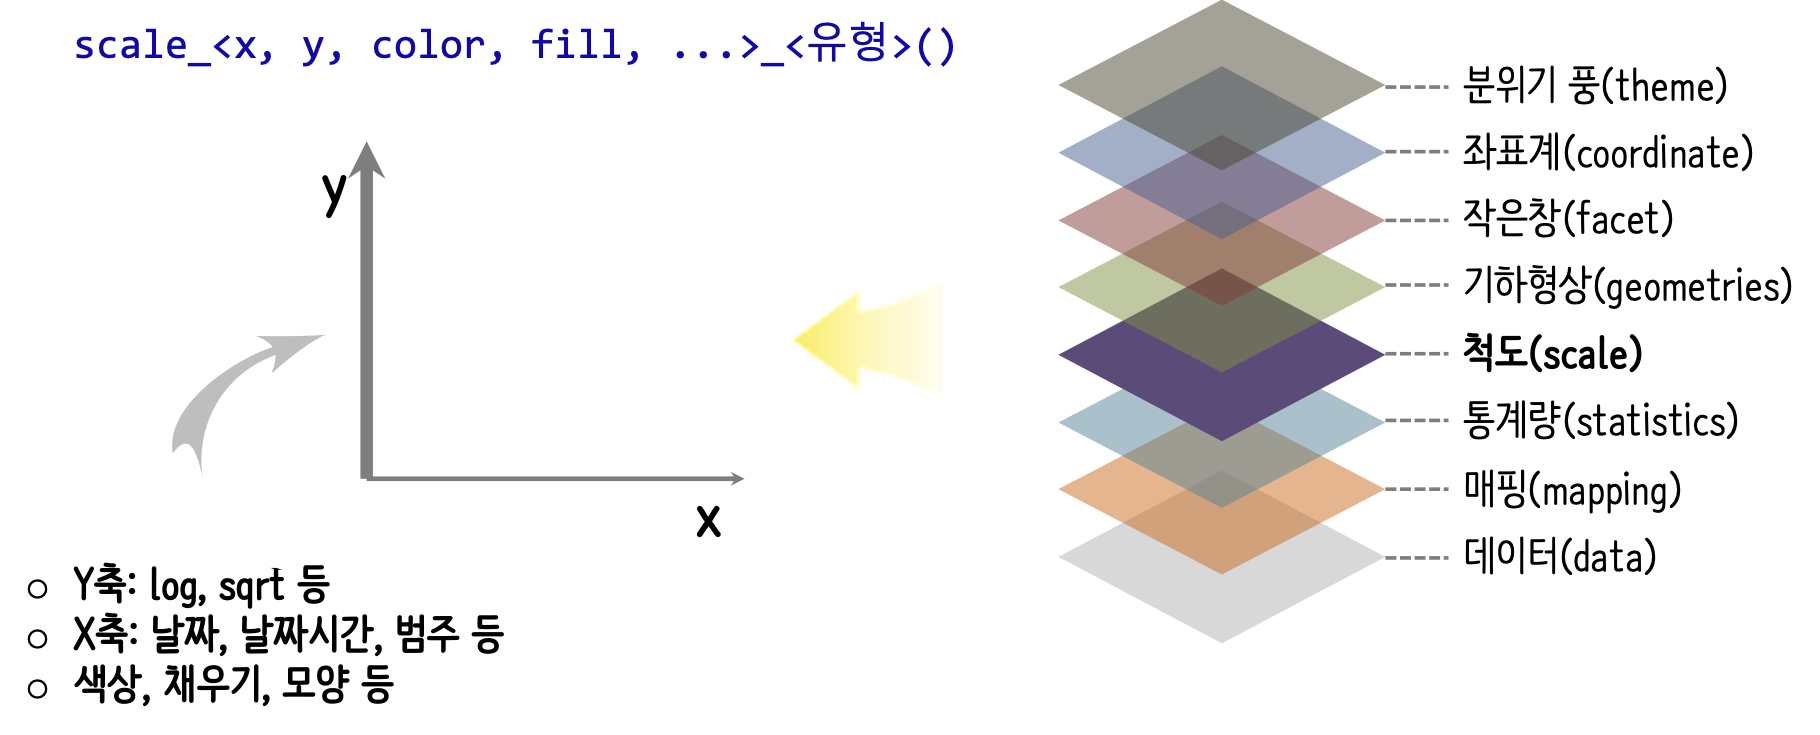
\includegraphics[width=1\textwidth,height=\textheight]{assets/images/ggplot-scales.png}
\caption{\texttt{aes} 매핑된 축 척도지정}
\end{figure}

\hypertarget{ggplot2-steps-geometries}{%
\subsection{기하형상(geometries)}\label{ggplot2-steps-geometries}}

예를 들어, 범주형 변수를 \texttt{aes()}로 지정하고 이를 적절한 그래프로 표현하기 위한 결정과정으로 \texttt{geom\_*()} 방식으로 원그래프, 막대그래프, 점그래프 등으로 변수를 시각화객체로 지정한다.

\begin{figure}
\centering
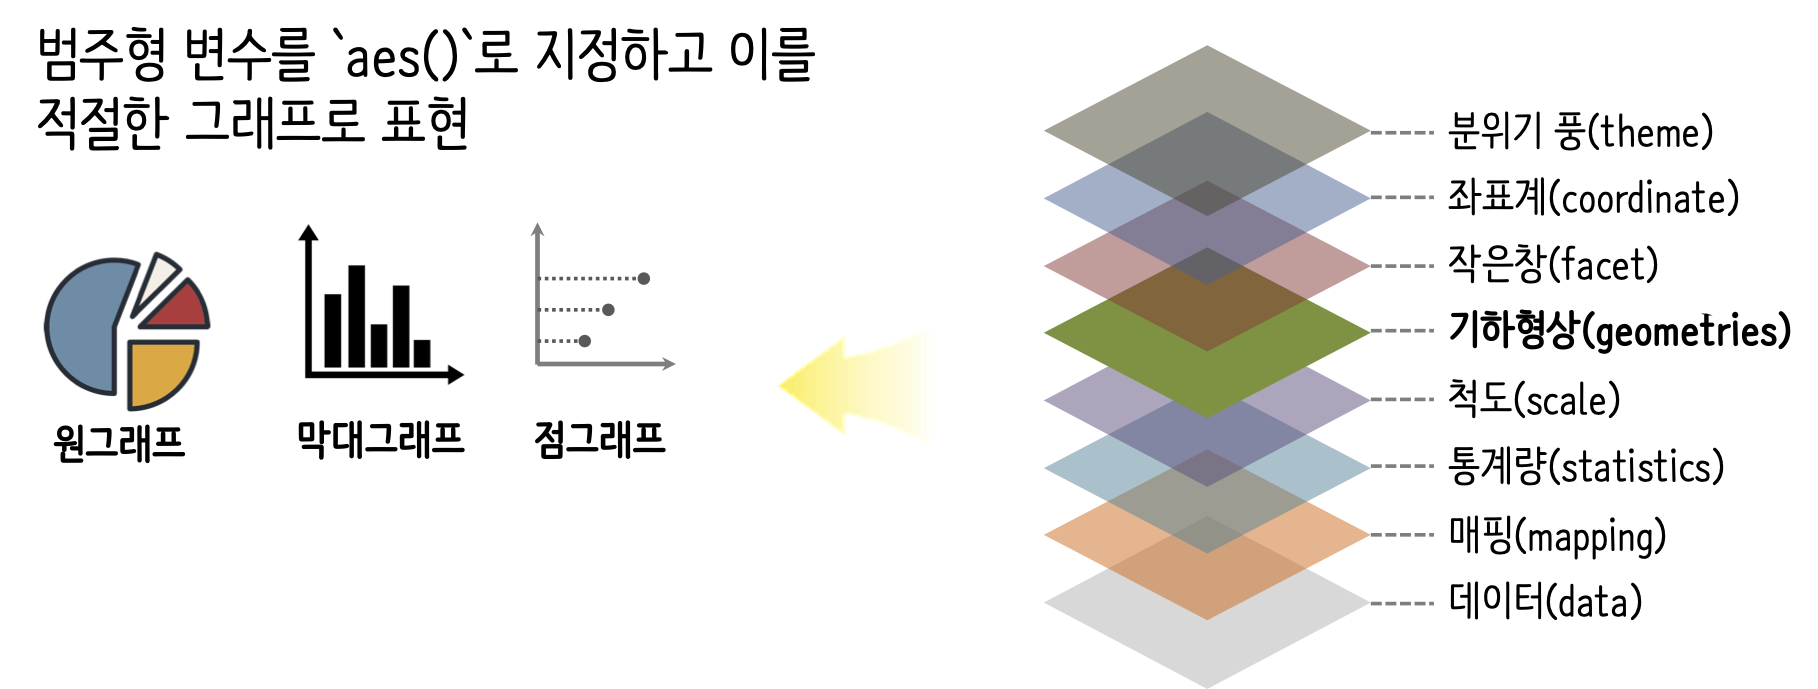
\includegraphics[width=1\textwidth,height=\textheight]{assets/images/ggplot-geometries.png}
\caption{기하형상 지정}
\end{figure}

\hypertarget{ggplot2-steps-facet}{%
\subsection{작은 창(facet)}\label{ggplot2-steps-facet}}

원본 데이터를 그룹으로 쪼개 작은 창에 동일한 시각화 객체를 표현하는 방법으로 다차원 데이터를 차원별로 나눠 볼 수 있다. 중요한 점은 각 작은 창이 동일한 유형의 그래프라는 점이 중요하다.

\begin{figure}
\centering
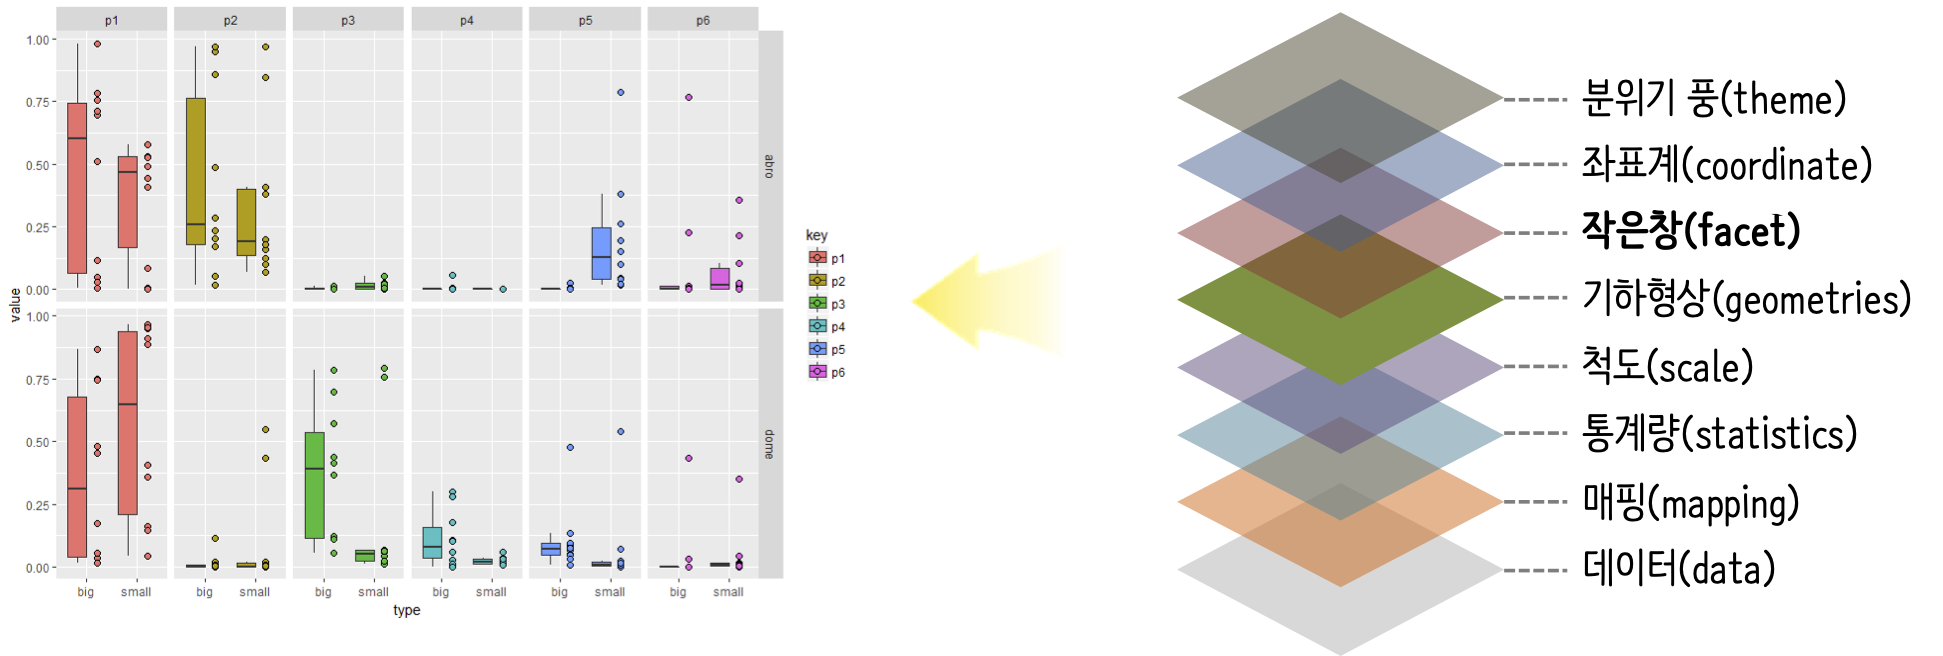
\includegraphics[width=1\textwidth,height=\textheight]{assets/images/ggplot-facet.png}
\caption{그룹으로 쪼갠 작은 창(facet)}
\end{figure}

\hypertarget{ggplot2-steps-coordinate}{%
\subsection{좌표계(coordinate)}\label{ggplot2-steps-coordinate}}

깔끔한 데이터를 그래프에 매칭하여 시각화한 후에 경우에 따라서 좌표계를 변경할 경우가 있다. \texttt{coord\_fixed()}, \texttt{coord\_polar()}, \texttt{coord\_flip()} 등을 사용해서 특정 영역 확대, 데카르트 좌표계에서 극좌표계, X-Y 축 변경 등의 작업을 수행할 수 있다.

\begin{figure}
\centering
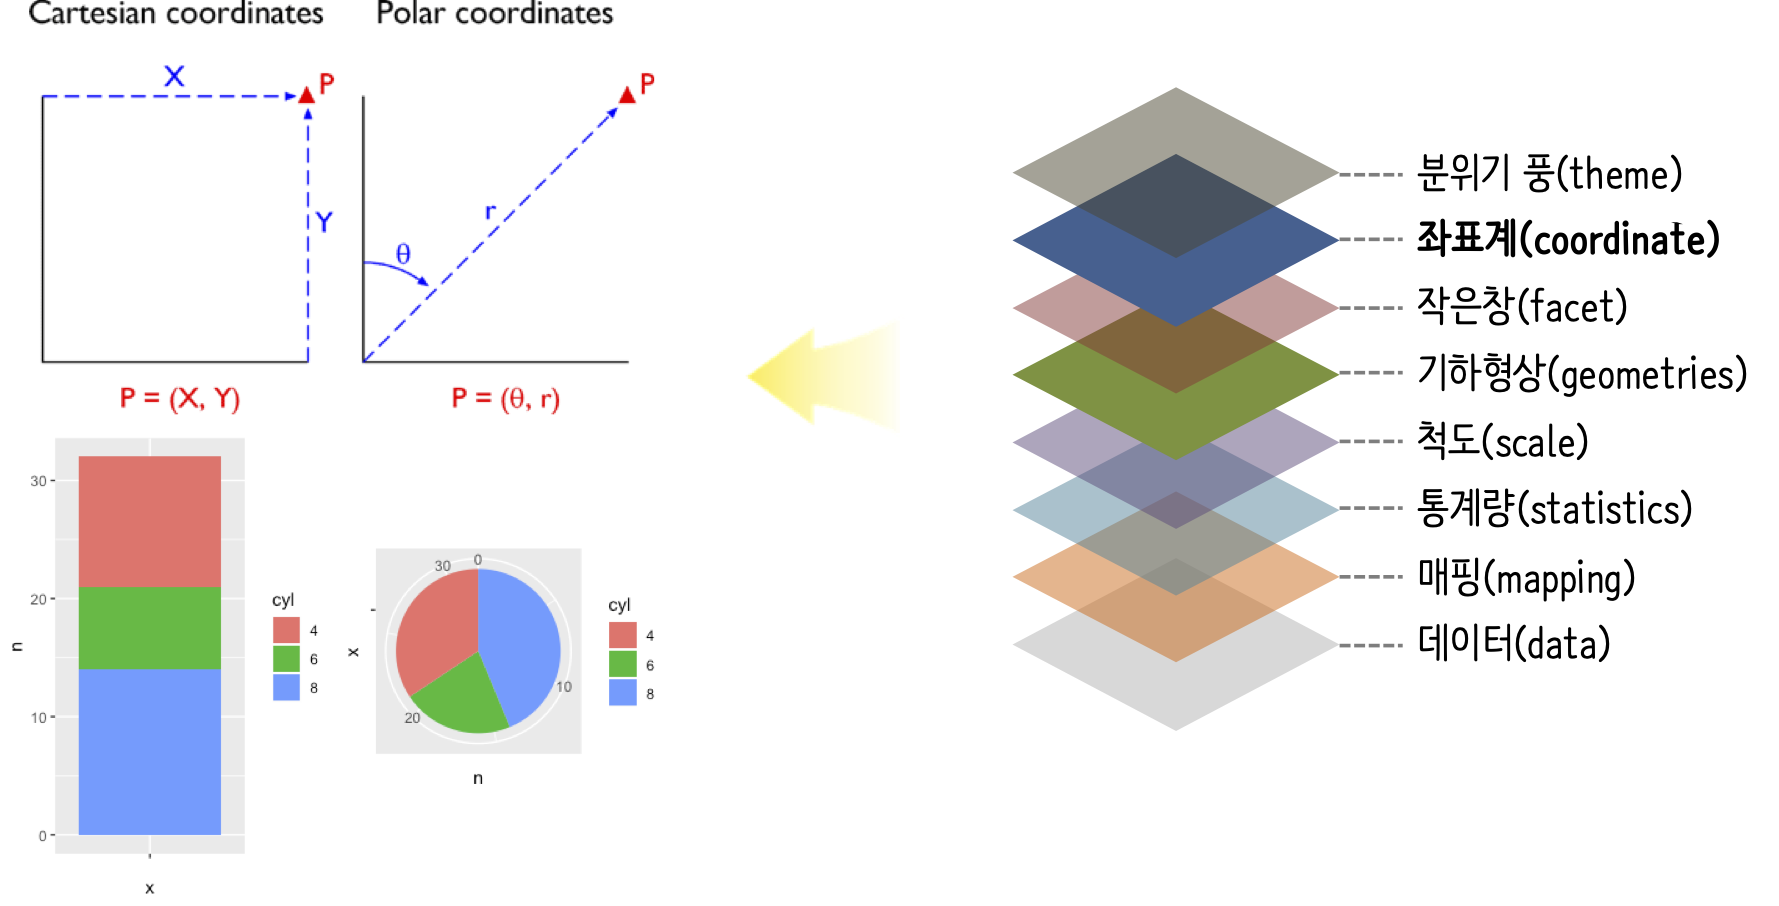
\includegraphics[width=1\textwidth,height=\textheight]{assets/images/ggplot-coordinate.png}
\caption{좌표계 변환}
\end{figure}

\hypertarget{ggplot2-steps-theme}{%
\subsection{분위기 풍(theme)}\label{ggplot2-steps-theme}}

분위기 풍(theme)은 앞선 깔끔한 데이터를 시각화 객체로 변환시키는 과정과 아무런 연관이 없다. 대신 외양을 보기좋게 하는 역할을 수행한다. 즉, 시각화에 알맞는 색상 팔레트를 적용시키고, 글꼴을 바꾸는 작업이 여기에 해당된다.

\begin{figure}
\centering
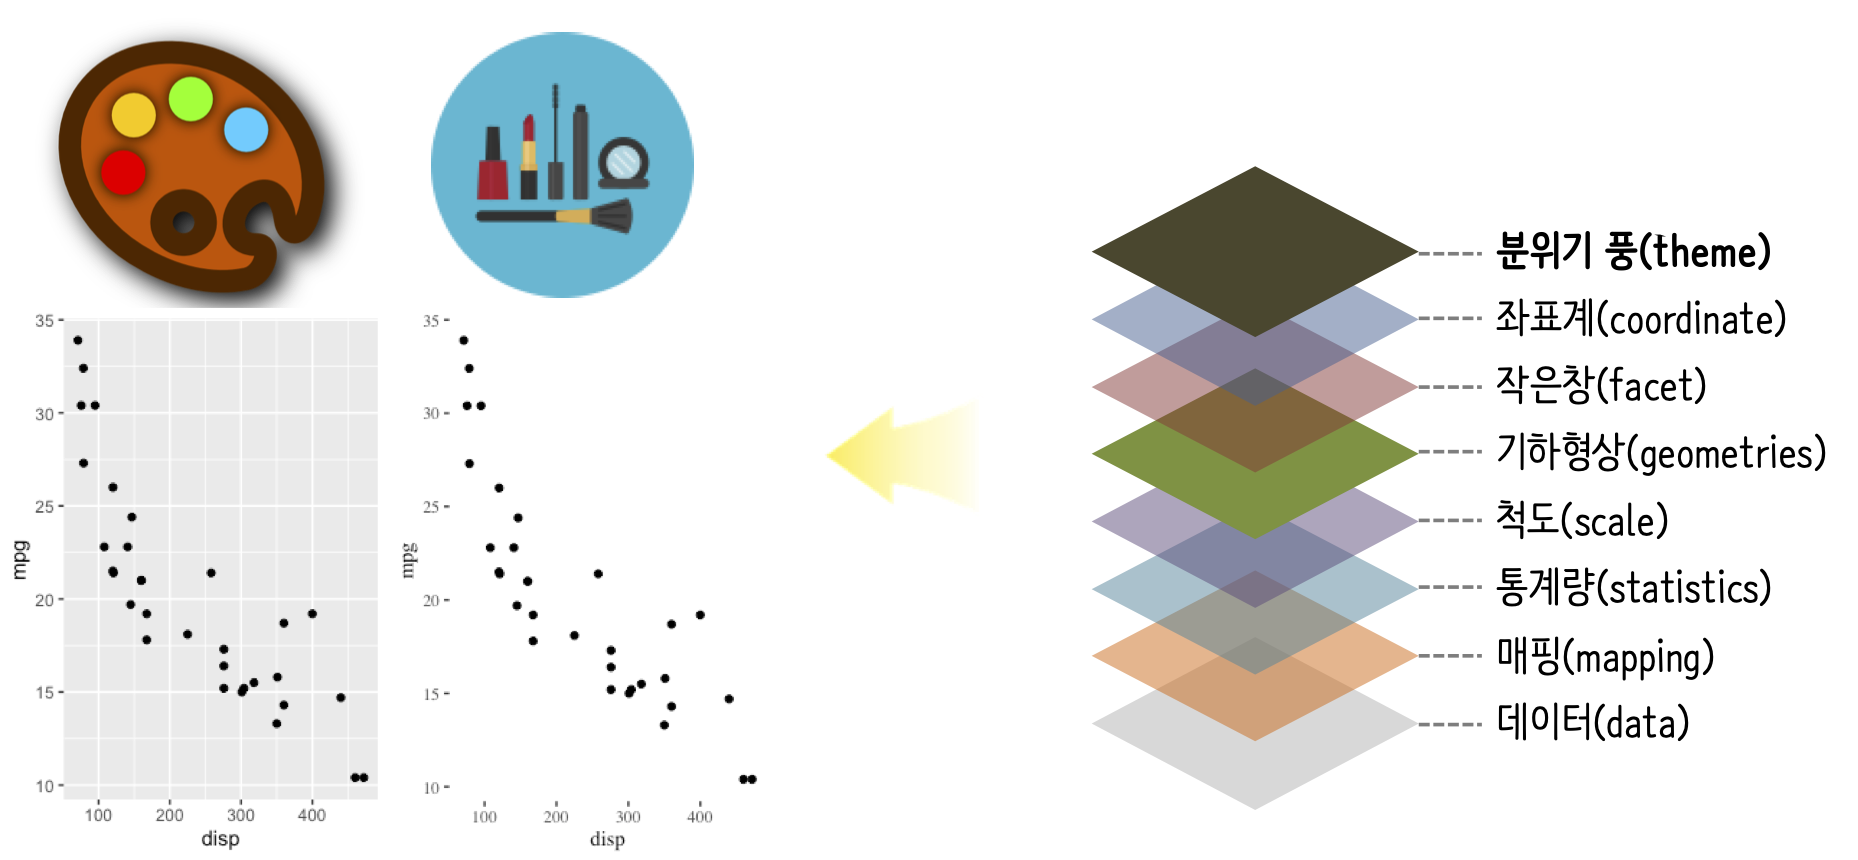
\includegraphics[width=1\textwidth,height=\textheight]{assets/images/ggplot-theme.png}
\caption{\texttt{tufte} 분위기 풍(theme)}
\end{figure}

\begin{center}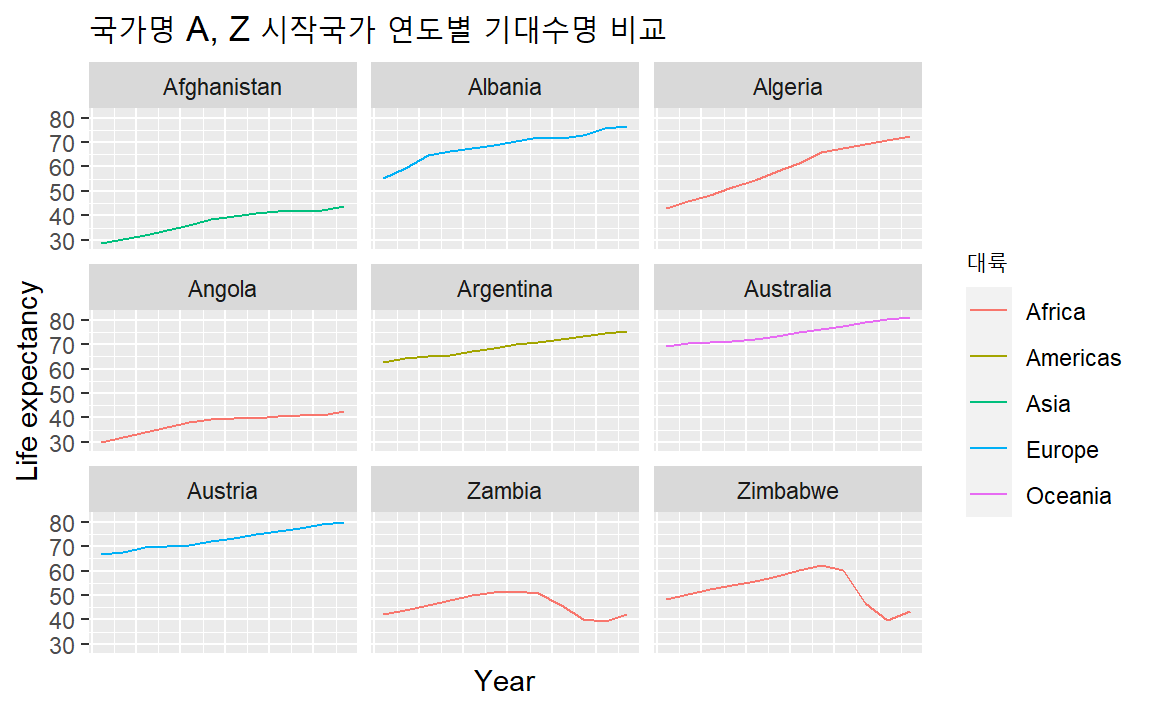
\includegraphics{viz-ggplot_files/figure-latex/ggplot-theme-1} \end{center}

\hypertarget{ggplot2-steps-extension}{%
\section{\texorpdfstring{\texttt{ggplot} 확장}{ggplot 확장}}\label{ggplot2-steps-extension}}

기본 \texttt{ggplot} 그래프 객체를 갖게 되면 2개 이상의 그래프를 합치거나 배열을 달리하고,
강조를 하고 주석(annotation)을 달고 애니메이션과 인터랙티브 기능을 추가하여 확장시킬 수 있다.

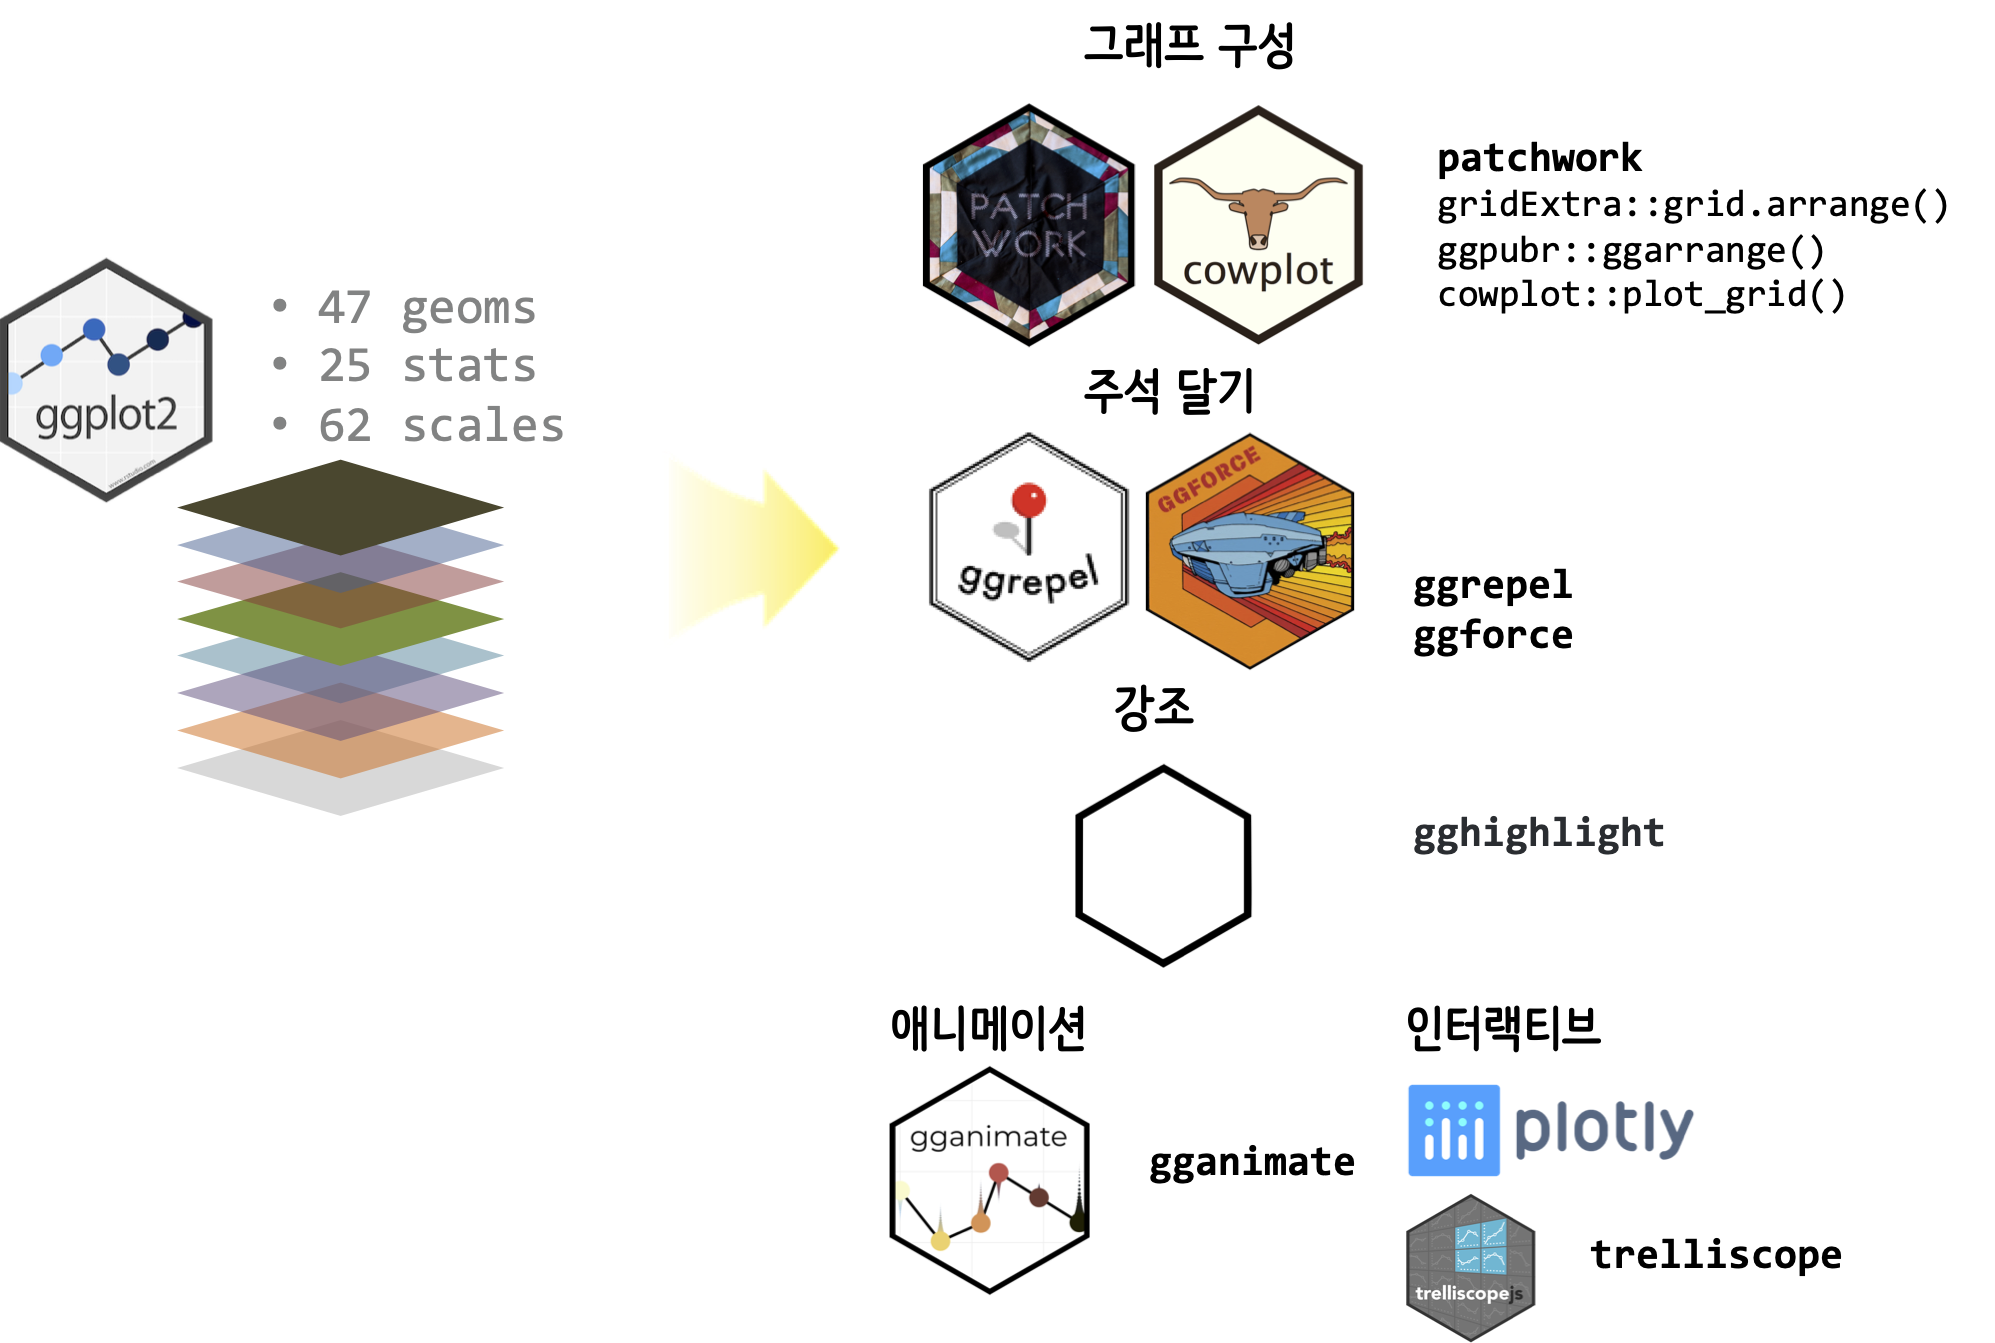
\includegraphics[width=1\textwidth,height=\textheight]{assets/images/ggplot-extension.png}

\hypertarget{ggplot-pattern}{%
\chapter{시각화 패턴}\label{ggplot-pattern}}

\hypertarget{gghighlight-timeseries}{%
\section{라벨 붙은 시계열}\label{gghighlight-timeseries}}

시계열 데이터를 제작하게 되면 추세를 파악할 수 있지만 결국 그래서 가장 최근 값이 어떻게 되는지 관심이 많다.
이런 사용자 요구를 맞추는데 시계열 데이터 마지막 시점에 라벨값을 붙이게 되면 가독성도 좋아진다.
기본적인 작업흐름은 데이터셋에서 가장 최근 관측점을 뽑아서 별도 데이터프레임으로 저장하고
이를 \texttt{geom\_text()} 혹은 \texttt{geom\_text\_repel()} 함수를 사용해서 해결한다.

BLOGR 님이 작성한 \href{https://drsimonj.svbtle.com/label-line-ends-in-time-series-with-ggplot2}{Label line ends in time series with ggplot2} 코드를 참조하여 \texttt{ggplot}으로 코드를 작성한다.

\begin{center}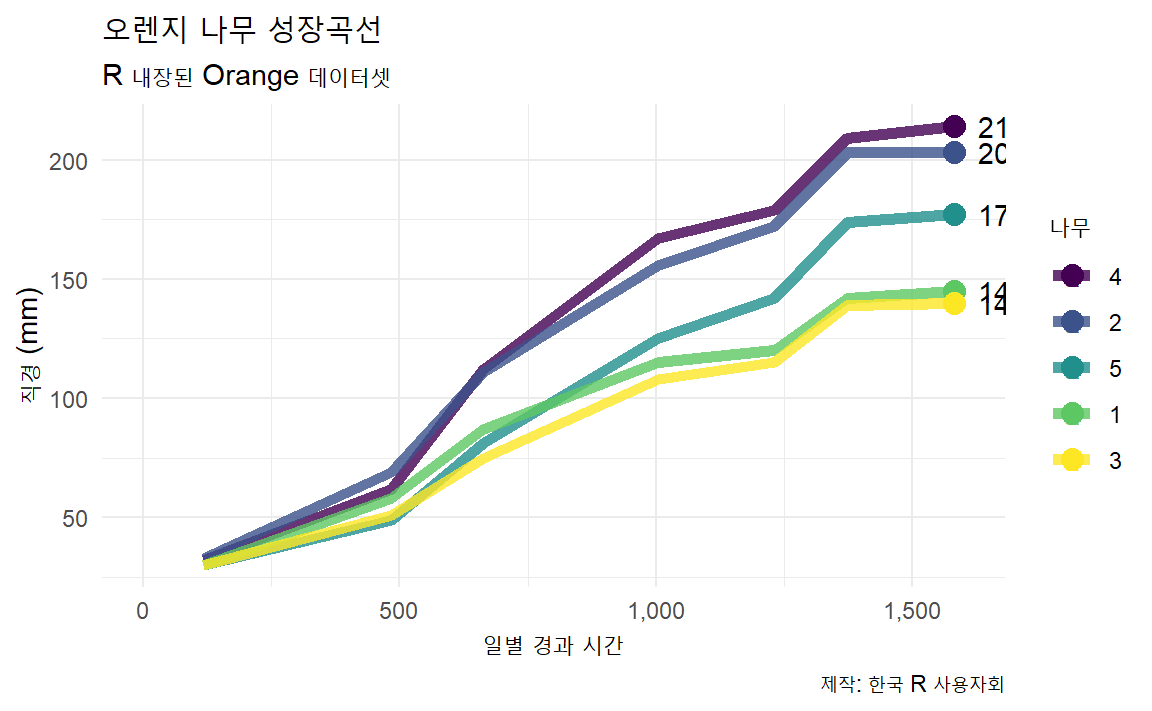
\includegraphics{viz-pattern_files/figure-latex/best-viz-label-1} \end{center}

\hypertarget{gghighlight-barplot-color}{%
\section{막대그래프 그룹별 색상}\label{gghighlight-barplot-color}}

RStudio를 거쳐 IBM에서 근무하고 있는 Alison Presmanes Hill 의 GitHub 저장소에 공개된 TV 시리즈 데이터를 사용해서 막대그래프를 작성할 때 그룹별 색상을 적용하여 가시성을 높인다. TV 시리즈별 색상을 달리할 경우 \texttt{RColorBrewer} 패키지 생상 팔레트를 범주형에 맞춰 각 시리즈별로 가장 잘 구분될 수 있도록 색상을 칠해 시각화를 한다.

\begin{center}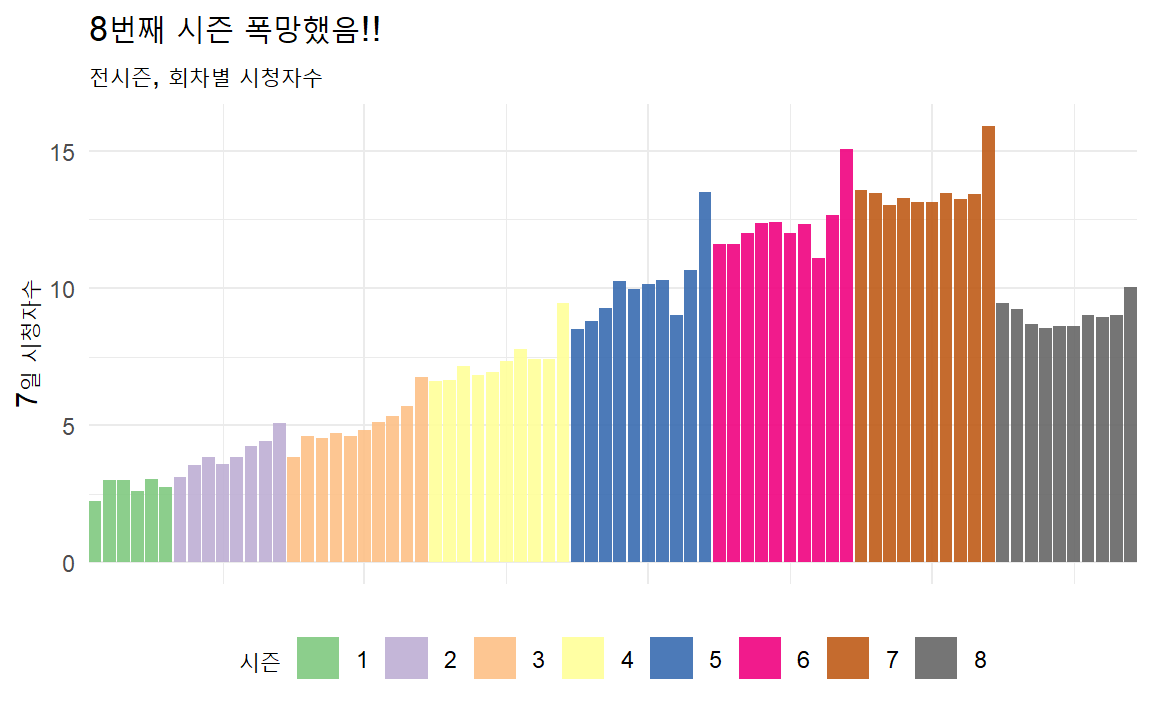
\includegraphics{viz-pattern_files/figure-latex/best-viz-barbplot-color-1} \end{center}

\hypertarget{gghighlight-trend-line-label}{%
\section{추세선 강조 + 라벨}\label{gghighlight-trend-line-label}}

시각화의 백미는 아무래도 대조와 비교를 통해 강한 인상을 주는 것이다.
앞선 \texttt{ratings} TV 시리즈 시청자 평가 데이터를 대상으로 추세선에 강조를 넣고 라벨 텍스트도 넣어
하이라이트 강조 그래프를 작성해보자.
\texttt{geom\_line()}을 두개 포함시켜 강조하고하는 색상을 별도로 지정하고 선굵기도 달리한다.
라벨도 동일한 방법으로 \texttt{geom\_text()}를 두개 포함시켜 강조하고자하는 색상과 글꼴크기도 달리 지정한다.

\begin{center}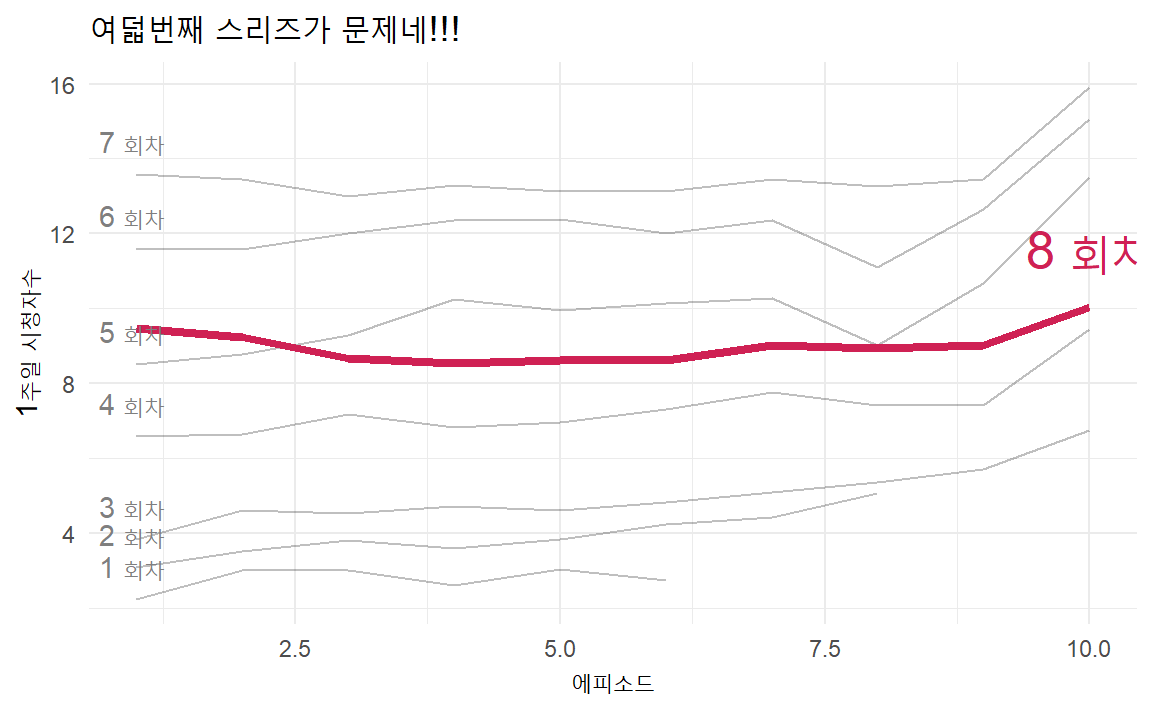
\includegraphics{viz-pattern_files/figure-latex/best-viz-trend-line-1} \end{center}

\hypertarget{gghighlight-barplot-color}{%
\section{롤리팝(lolli-pop) 그래프}\label{gghighlight-barplot-color}}

롤리팝(Lollipop) 사탕 그래프는 막대그래프와 클리블랜드 점그래프를 합성한 것으로 한축에는 연속형, 다른 한축에는 범주형을 두고 사용자의 관심을 점그래프로 집중시키는데 효과적이다. 단순히 막대그래프를 제작하는 것과 비교하여 임팩트있는 시각화를 가능하게 한다.

제작순서는 막대그래프 → 점그래프 → 롤리팝 그래프로 뼈대 골격을 만들어 나간다.
대략 골격이 제작되고 나면 외양과 필요한 경우 값도 텍스트로 넣어 시각화 제품을 완성한다.
롤리팝 사탕 그래프를 작성할 때 \texttt{geom\_point()}를 사용해서 롤리팝 사탕을 제작하고,
\texttt{geom\_sgement()} 함수를 사용해서 사탕 막대를 그린다. 이때 막대 사탕의 시작과 끝을
시작은 \texttt{x}, \texttt{y}에 넣어주고 끝은 \texttt{xend}와 \texttt{yend}에 넣어 마무리한다.

데이터는 \texttt{ggplot2}에 내장된 \texttt{midwest} 데이터를 사용하자. \texttt{midwest} 데이터셋은
2000년 미국 중서부 센서스 데이터로 인구통계 조사가 담겨있다.
\texttt{percollege} 변수는 카운티(우리나라 군에 해당) 별 대학졸업비율을 나타낸다.

\begin{center}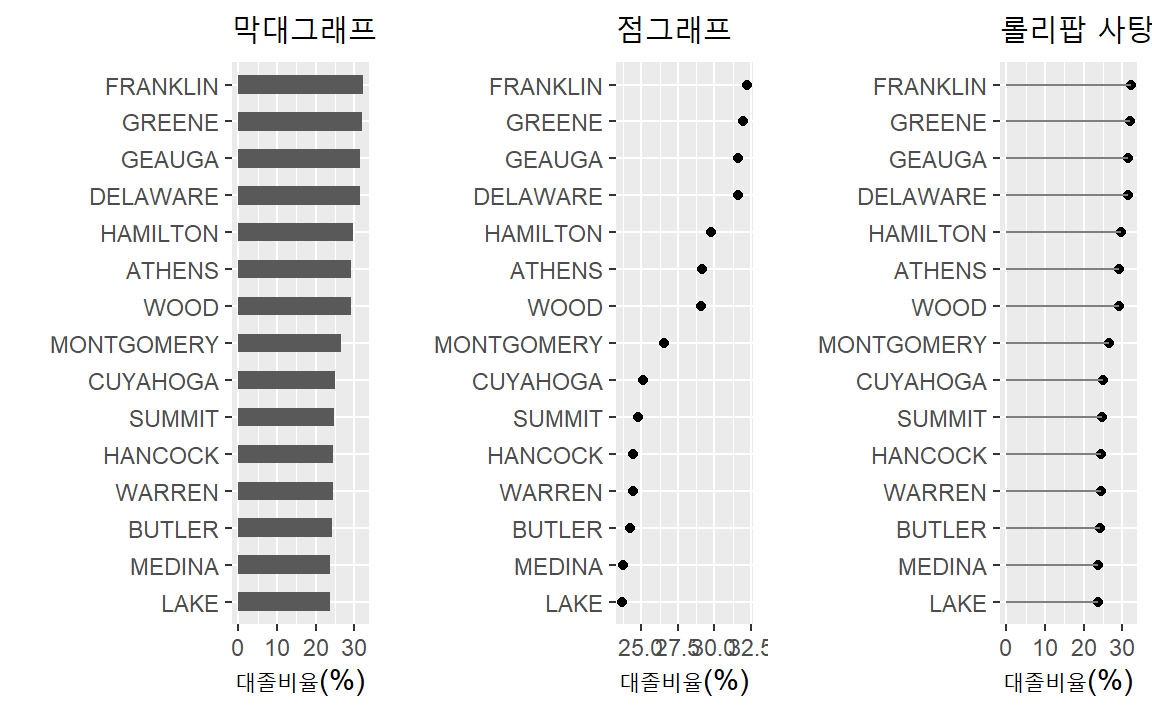
\includegraphics{viz-pattern_files/figure-latex/best-viz-lolli-pop-1} \end{center}

한발더 나아가, 평균값에서 얼마나 차이가 있느냐를 롤리팝 그래프로 시각화하는 패턴이 많이 사용된다.
이를 위해서, 앞서와 마찬가지로 15개 카운티를 뽑아내고 평균을 구하고 평균이상, 평균이하에 대한 요인(factor)도 함께 만들어낸다.
반영한다.

\begin{center}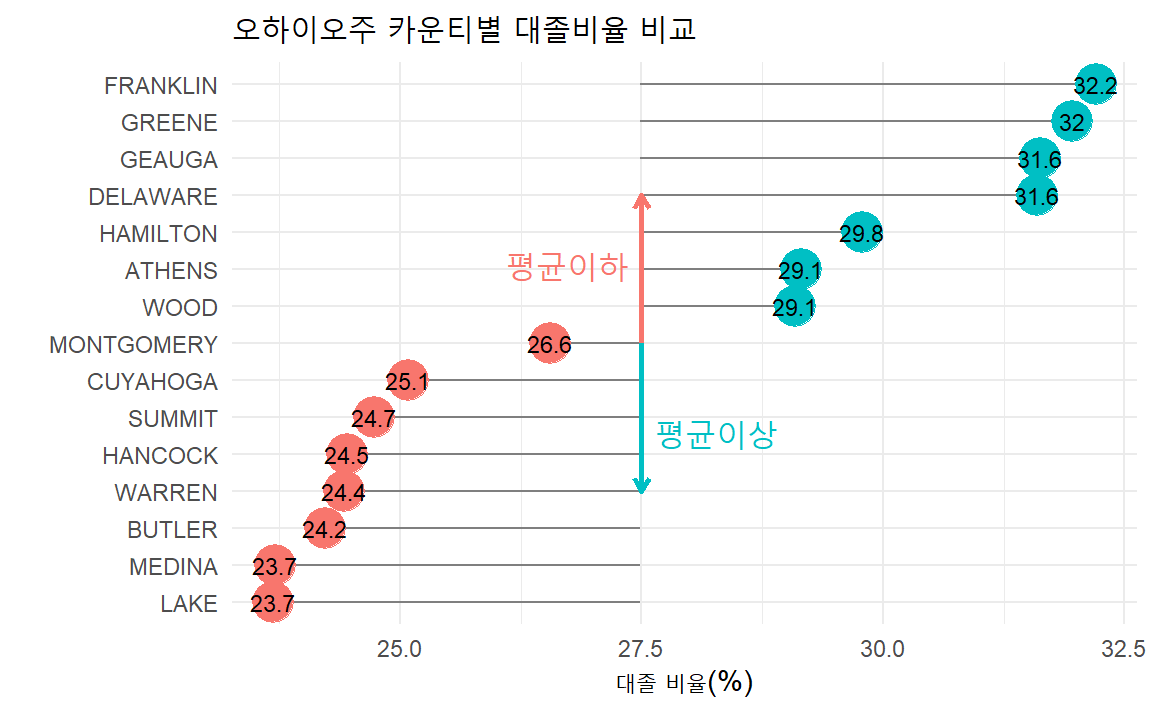
\includegraphics{viz-pattern_files/figure-latex/best-viz-lolli-pop-polish-1} \end{center}

\hypertarget{gghighlight-dumbbel-plot}{%
\section{아령(dumbbell) 그래프}\label{gghighlight-dumbbel-plot}}

두시점을 비교하여 전후를 비교한다던가 두 지역을 비교할 때 아령 그래프는 매우 효과적이다.
TV 시리즈별로 회차를 달리하여 첫번째와 가장 마지막 시청자수를 비교하여 시각화하는데 아령(dumbbell) 그래프가 적절한 예시가 될 것으로 보인다. 이를 위해서 \texttt{ggplot()}에 들어가는 자료형을 미리 준비하고 이에 맞춰 \texttt{geom\_line()}과 \texttt{geom\_point()}를 결합시켜 시각화한다.

\begin{center}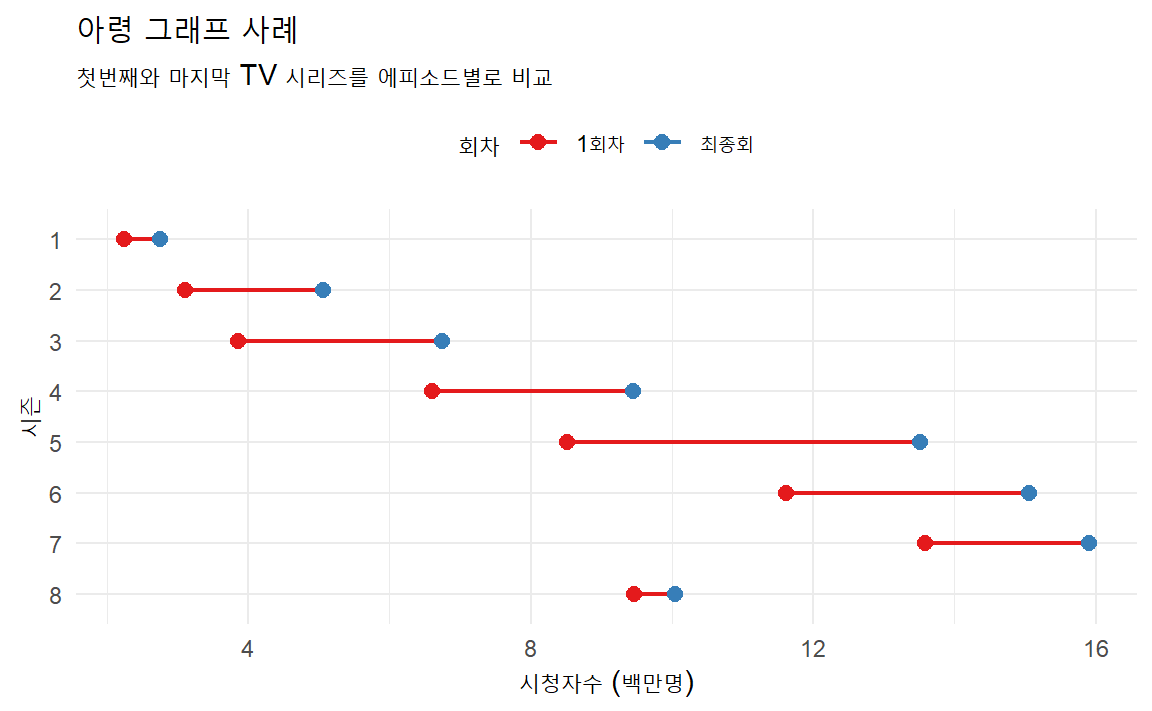
\includegraphics{viz-pattern_files/figure-latex/best-viz-dumbbell-plot-1} \end{center}

\hypertarget{gghighlight-slope-plot}{%
\section{경사(Slope) 그래프}\label{gghighlight-slope-plot}}

아령 그래프를 제작한 동일한 데이터를 \href{https://www.edwardtufte.com/bboard/q-and-a-fetch-msg?msg_id=0003nk}{\texttt{터프티(tufte)} 스타일 경사그래프}로 구현하면
시즌별 첫회와 최종회 시청자수 비교를 좀더 직관적으로 만들 수 있다.

\texttt{ggplot}의 기본기능을 활용하여 경사그래프를 시각화하고 강조하고자 하는 시즌을
색상을 달리하여 표현한다. 이를 통해 1\textasciitilde7번째 시즌은 1회차 시청율은 낮으나 최종회는 높게
마무리된 것을 알 수 있고, 더불어 시즌이 진행될 수록 1회차 시청율도 높아지고 있었다.
하지만 8번째 시즌은 다른 시즌과 달리 낮게 시작했고 최종회 시청률도 크게 나아지지 않은 것을
한눈에 파악할 수 있다.

\begin{center}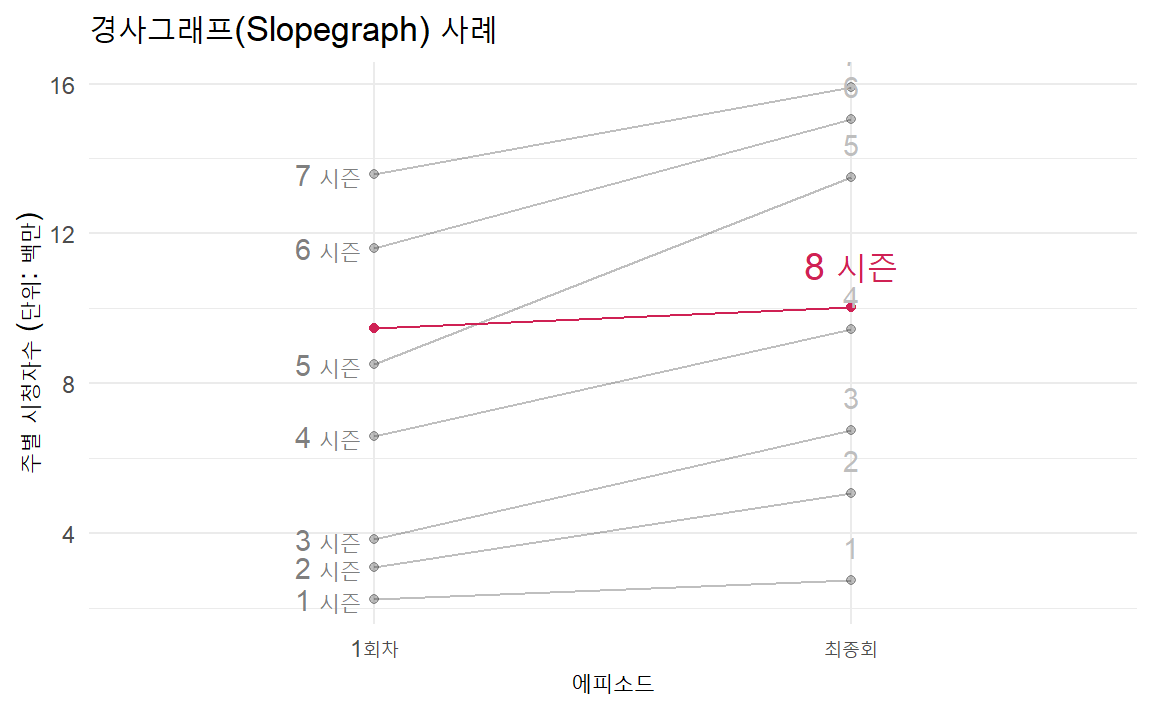
\includegraphics{viz-pattern_files/figure-latex/best-viz-slope-plot-base-1} \end{center}

경사그래프를 제작하고는 싶으나 전반적으로 시간이 더 필요하신 분을 위해
\href{https://github.com/leeper/slopegraph}{\texttt{slopegraph}} 패키지가 있다.

\texttt{slopegraph}는 Base 그래픽을 기본으로 삼고 있어 자료구조도 \texttt{rownames}를 갖는 전통적인 데이터프레임이다.
기본 Base 그래픽을 염두에 두고 상기 TV 연속물 경사그래프를 다음과 같이 작성할 수 있다.

\begin{center}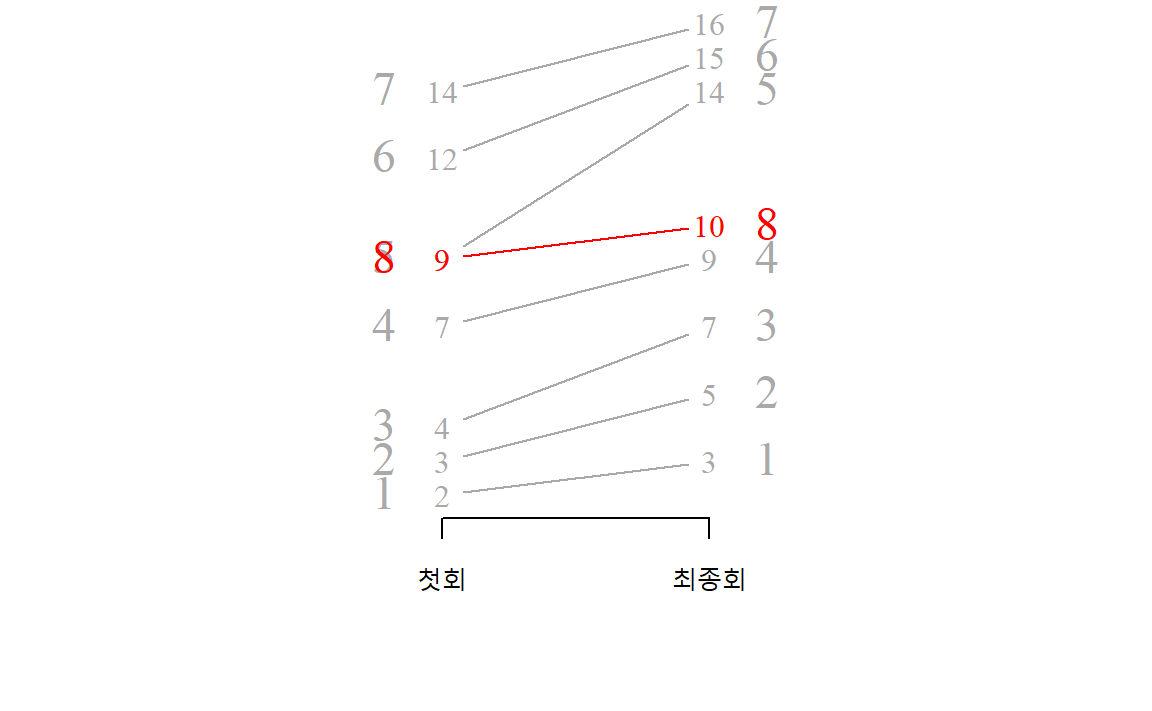
\includegraphics{viz-pattern_files/figure-latex/best-viz-slope-plot-slopegraph-series-1} \end{center}

\texttt{slopegraph()} 함수 대신 \texttt{ggslopegraph()} 함수를 사용하게 되면 \texttt{ggplot()}으로도 시각화를 할 수 있다.
\texttt{slopegraph()} 함수는 자료구조가 직관적이라 처음 시각화를 하는 분에게 적절한 듯 보인다.
따라서, 앞서 \texttt{ggplot} 기반 경사그래프를 제작하고자 하는 경우 \texttt{ggslopegraph()}을 통해서도 \texttt{ggplot} 나머지 기능을 그대로 적용 가능하다.

\begin{center}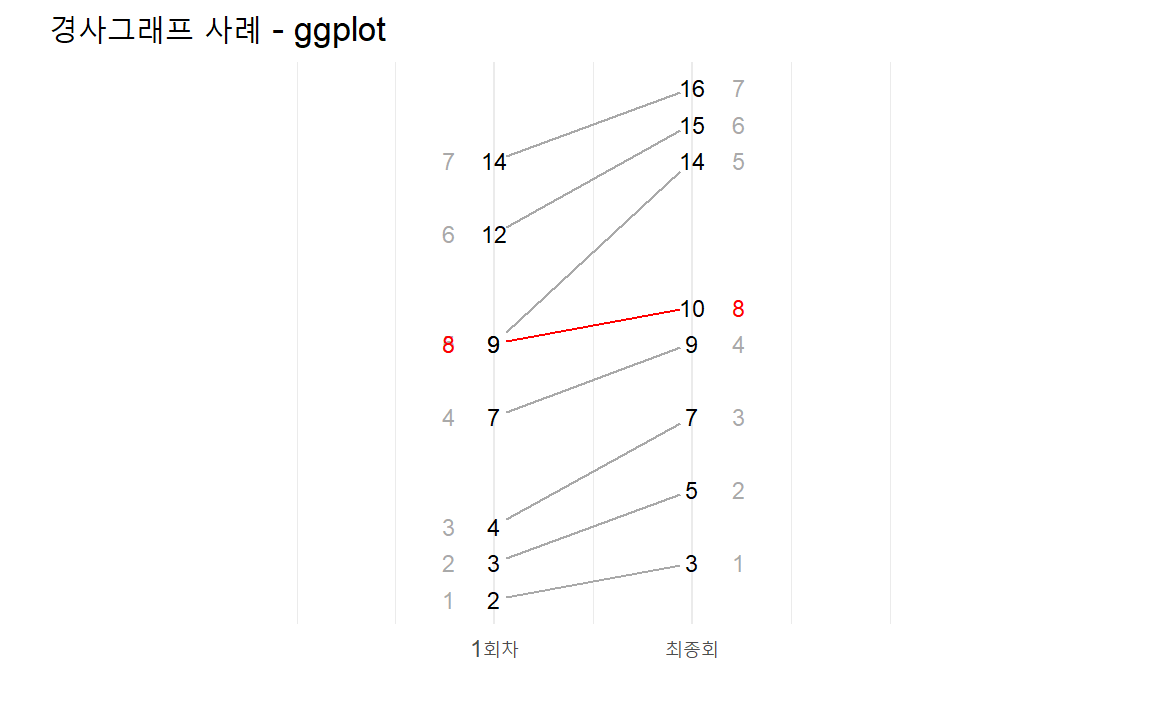
\includegraphics{viz-pattern_files/figure-latex/best-viz-slope-plot-ggslopegraph-series-1} \end{center}

\hypertarget{uxc0acuxb840}{%
\chapter*{사례}\label{uxc0acuxb840}}
\addcontentsline{toc}{chapter}{사례}

\hypertarget{case-journalism}{%
\chapter{데이터 저널리즘}\label{case-journalism}}

\hypertarget{case-worldcup}{%
\chapter{러시아 월드컵}\label{case-worldcup}}

\hypertarget{case-corona}{%
\chapter{코로나19}\label{case-corona}}

\begin{itemize}
\tightlist
\item
  GitHub 저장소 : \href{https://github.com/clauswilke/dataviz}{clauswilke/dataviz}
\end{itemize}

  \bibliography{book.bib,packages.bib}

\end{document}
